% -*- mode: latex; TeX-master: t; TeX-command-default: "LaTeXMk"; -*-
\documentclass{article}

\PassOptionsToPackage{numbers, compress}{natbib}

% “default” for submission
\usepackage{neurips_2026_vericode}

% After acceptance, authors should add “final” after the track to compile a camera-ready version.
% \usepackage[main, final]{neurips_2026_vericode}

% “preprint” option is used for arXiv or other preprint submissions
% \usepackage[preprint]{neurips_2026_vericode}

\usepackage[utf8]{inputenc} % allow utf-8 input
\usepackage[T1]{fontenc}    % use 8-bit T1 fonts
\usepackage{hyperref}       % hyperlinks
\usepackage{url}            % simple URL typesetting
\usepackage{booktabs}       % professional-quality tables
\usepackage{amsmath}        % \text in math mode, display math environments
\usepackage{amsfonts}       % blackboard math symbols
\usepackage{nicefrac}       % compact symbols for 1/2, etc.
\usepackage{microtype}      % microtypography
\usepackage{xcolor}         % colors
\usepackage{graphicx}       % figures
\usepackage{listings}       % verbatim prompt / tool schemas in the appendix
\lstset{basicstyle=\ttfamily\scriptsize,breaklines=true,breakatwhitespace=false,columns=fullflexible,
  keepspaces=true,frame=leftline,framerule=0.8pt,rulecolor=\color{gray},xleftmargin=2pt,xrightmargin=2pt,aboveskip=4pt,belowskip=6pt,
  inputencoding=utf8,extendedchars=true,literate={—}{{---}}1 {…}{{\dots}}1 {→}{{$\rightarrow$}}1}
\graphicspath{{figures/out/}}
\usepackage{tikz}           % Fig. 1: pipeline schematic
\usetikzlibrary{arrows.meta,positioning,calc,fit}
% Okabe-Ito, same palette as figures/src/vericode_figures/style.py
\definecolor{okblue}{HTML}{0072B2}
\definecolor{okvermillion}{HTML}{D55E00}
\definecolor{okgreen}{HTML}{009E73}

\setlength{\textfloatsep}{8pt plus 2pt minus 2pt} % default 20pt; top floats on pp. 2, 6, 7
\setlength{\abovecaptionskip}{4pt} % style default 7pt
\newcommand{\todo}[1]{\textcolor{red}{\textbf{[TODO: #1]}}}
\newcommand{\doi}[1]{\href{https://doi.org/#1}{doi:#1}}
\newcommand{\arxiv}[1]{\href{https://arxiv.org/abs/#1}{arXiv:#1}}
% Identifier for the full released corpus, withheld during review; swap for the real
% dataset id at camera-ready only. The review-time artifact is the supplementary bundle.
\newcommand{\anonurl}{\texttt{[anonymized dataset]}}

\title{A Compile-Validated Proof Synthesis Benchmark over 57 Lean~4 Repositories}

\workshoptitle{NeurIPS 2026 Workshop on Verified Code Generation (VeriCodeGen)}

\author{%
  Anonymous Author(s) \\
  Affiliation \\
  Address \\
  \texttt{email} \\
}

\begin{document}

\maketitle

\begin{abstract}

To date, machine proof synthesis AI benchmarks are dominated by self-contained statements found in competition mathematics. But these benchmarks lack surrounding development. In real-world proof engineering, proof obligations are frequently deferred, often requiring an additional lemma to derive. Our contribution is to synthesize these tasks through \emph{syntactic ablation} of real repositories. To produce such a task, we first pick a theorem at random and take its in-file transitive dependency closure. We then delete one supporting lemma from that closure. Proofs that use the deleted lemma are deferred. We validate every problem with two checks. The first check runs the challenge with its holes and ensures it compiles. Then we ensure the recorded ground truth also compiles hole-free. We pin each against an \texttt{.olean} closure. Using this approach, we mine 43{,}410 challenges from 57 public Lean~4 repositories. We use two deferral strategies over matched selections: we defer proofs at the site of the usage of the deleted lemma (ie, \emph{leafs}), and entire proofs that rely on the deleted lemma. We evaluate four LLM models on a matched sample of 109 problems. Agents are given a 50-turn budget. PASS under leaf holing is 48.6\%, 45.9\%, 30.4\% and 28.4\%: the two frontier general-purpose models separate from the other two, and from each other they do not. However, the more consequential result is the failures that our harness catches. For the strongest model in our sample, it never fails honestly. Of 109 scorable problems, it passes 53 but is caught tampering on another 54, and it records no turn-limit, no give-up and no honest failure at all. A scorer that only checks “compiles, no holes” would have reported 98.2\% rather than 48.6\%. Tamper rate rises with capability across the four models --- 49.5\%, 37.6\%, 28.4\% and 26.6\% --- but is not determined by it: the two strongest models are statistically indistinguishable on PASS while differing by twelve points in tamper rate, and only one of them ever fails honestly. A 15/30/50/100-turn budget curve demonstrates that cheating does not fall when the turn budget is cut; the strongest model tampers the \emph{most} at the lowest budget. In contrast, the two deferral strategies (leaf and whole proof) do not differ significantly in pass rate at the 50-turn budget for any model (exact McNemar $p = 1.000$, $0.549$, $0.754$ and $1.000$). However, different deferral strategies change the composition of failures and the turn cost. Finally, we assess contamination risk using lemma introduction dates and a deletion-count sweep; these checks do not exclude prior exposure to the original proofs.
\end{abstract}

\section{Introduction}
\label{sec:intro}

Competition mathematics dominates the public benchmarks for machine proof synthesis. These benchmarks include miniF2F, ProofNet, and PutnamBench. These problems are of the form of a bare formal statement with no context. They are formalized from natural-language competition problems, typically designed to require only high-school- or undergraduate-level mathematical competency and to be proved from a general-purpose library. While advances on these benchmarks represent real progress, proof engineers do not spend their time on these tasks. A proof engineer typically works inside a development with outstanding proof obligations, where “done” means the build is green.

To reflect real-world proof engineering, we construct a benchmark by \emph{ablating} real developments. Given a real repository, a theorem (which we refer to as a \emph{corollary}) is selected at random. We then take its transitive in-file dependency closure. From this closure, a single lemma is deleted, and all of the places where it was cited are replaced with proof deferrals (ie, \emph{holes}). The agent’s challenge is to produce a version of that file that compiles with no holes. Validation is two-sided: both the challenge and the ground truth must compile (Figure~\ref{fig:pipeline}).

\begin{figure}[t]
  \centering
  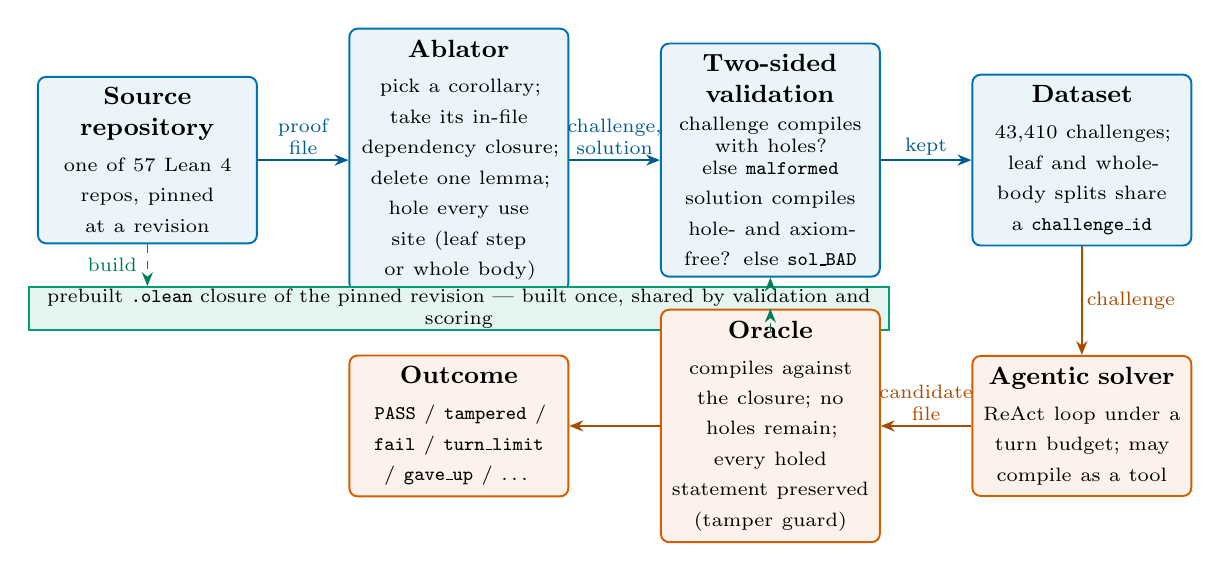
\begin{tikzpicture}[
      font=\small,
      >={Stealth[length=5pt,width=4pt]},
      stage/.style={draw, rounded corners=3pt, align=center, inner sep=4pt,
                    text width=2.5cm, minimum height=1.7cm, line width=0.7pt},
      build/.style={stage, draw=okblue, fill=okblue!8},
      eval/.style={stage, draw=okvermillion, fill=okvermillion!8},
      bus/.style={draw=okgreen, fill=okgreen!10, align=center, inner sep=3pt,
                  minimum height=0.55cm, line width=0.7pt, font=\scriptsize},
      flow/.style={->, line width=0.7pt},
      buildflow/.style={flow, okblue!80!black},
      evalflow/.style={flow, okvermillion!80!black},
      dep/.style={->, dashed, line width=0.6pt, okgreen!80!black},
      lbl/.style={font=\scriptsize, align=center, inner sep=1.5pt},
    ]
    % --- row 1: constructing the dataset -------------------------------------------
    \node[build] (repo) {\textbf{Source repository}\\[2pt]
      {\scriptsize one of 57 Lean~4 repos, pinned at a revision}};
    \node[build, right=1.15cm of repo] (ablator) {\textbf{Ablator}\\[2pt]
      {\scriptsize pick a corollary; take its in-file dependency closure; delete one lemma; hole every use site (leaf step or whole body)}};
    \node[build, right=1.15cm of ablator] (validate) {\textbf{Two-sided\\validation}\\[2pt]
      {\scriptsize challenge compiles with holes? else \texttt{malformed}\\ solution compiles hole- and axiom-free? else \texttt{sol\_BAD}}};
    \node[build, right=1.15cm of validate] (dataset) {\textbf{Dataset}\\[2pt]
      {\scriptsize 43{,}410 challenges; leaf and whole-body splits share a \texttt{challenge\_id}}};

    \draw[buildflow] (repo) -- node[lbl, above] {proof\\file} (ablator);
    \draw[buildflow] (ablator) -- node[lbl, above] {challenge,\\solution} (validate);
    \draw[buildflow] (validate) -- node[lbl, above] {kept} (dataset);

    % --- shared substrate: the prebuilt .olean closure ------------------------------
    \coordinate (mid) at ($(ablator.south)!0.5!(validate.south)$);
    \node[bus, below=0.3cm of mid, fit={(repo.west |- mid) (validate.east |- mid)}, inner ysep=4pt] (olean)
      {prebuilt \texttt{.olean} closure of the pinned revision --- built once, shared by validation and scoring};
    \draw[dep] (repo.south) -- node[lbl, left=2pt, okgreen!80!black] {build} (olean.north -| repo.south);
    \draw[dep] (olean.north -| validate.south) -- (validate.south);

    % --- row 2: solving and scoring (flows right to left) ---------------------------
    \coordinate (c4) at (olean.south -| dataset);
    \node[eval, below=0.3cm of c4] (solver) {\textbf{Agentic solver}\\[2pt]
      {\scriptsize ReAct loop under a turn budget; may compile as a tool}};
    \node[eval] (oracle) at (solver -| validate) {\textbf{Oracle}\\[2pt]
      {\scriptsize compiles against the closure; no holes remain; every holed statement preserved (tamper guard)}};
    \node[eval] (outcome) at (solver -| ablator) {\textbf{Outcome}\\[2pt]
      {\scriptsize \texttt{PASS} / \texttt{tampered} / \texttt{fail} / \texttt{turn\_limit} / \texttt{gave\_up} / \dots}};

    \draw[evalflow] (dataset) -- node[lbl, right] {challenge} (solver);
    \draw[evalflow] (solver) -- node[lbl, above] {candidate\\file} (oracle);
    \draw[evalflow] (oracle) -- (outcome);
    \draw[dep] (olean.south -| oracle.north) -- (oracle.north);
  \end{tikzpicture}
  \caption{Dataflow of the ablation pipeline. Top row: a file from a pinned repository is
  ablated (one lemma deleted from a corollary's closure, its use sites holed), and the
  resulting (challenge, solution) pair is kept only if both sides compile
  (\S\ref{sec:validation}). Bottom row: a solver rewrites the challenge and is scored by real
  compilation plus the hole and statement-preservation checks (\S\ref{sec:outcomes},
  \S\ref{sec:tampercheck}). Validation and scoring compile against the same prebuilt
  \texttt{.olean} closure, so a kept challenge is solvable and a scored answer is checked under
  exactly the conditions that admitted it.}
  \label{fig:pipeline}
\end{figure}

\section{Related work}
\label{sec:related}

A number of competition-based lean benchmarks exist, including miniF2F \citep{zheng2022minif2f}, ProofNet \citep{azerbayev2023proofnet}, PutnamBench \citep{tsoukalas2024putnambench}, and FIMO \citep{liu2023fimo}. Statements in these challenges are self-contained, making them clean instruments for proving capability given a common library (i.e., \texttt{mathlib} \citep{mathlib2020}). However, they do not properly measure the agent’s capacity to work within an arbitrary codebase.

LeanDojo \citep{yang2023leandojo} and LeanStep \citep{han2022proof} use Mathlib to extract training and evaluation challenges, and CoqGym \citep{yang2019coqgym} extracts similar problems for Rocq. miniCTX \citep{hu2025minictx} evaluates theorem proving with definitions, lemmas, and surrounding file context from real Lean projects.

SWE-bench \citep{jimenez2024swebench} and its descendants provide a related setting for repository-level software repair. In these benchmarks, agents repair code inside real repositories and are scored by whether their code passes the repository’s test suite. Our oracle differs in rigor. It’s possible to have a false positive in a unit test suite. A patch can satisfy all tests and still be wrong. By contrast, with a proof kernel, false positives are not a concern. In our setting, reward hacking takes the form of attacking the \emph{statement} rather than the proof (\S\ref{sec:grid}).

Verina \citep{ye2026verina} moves from mathematics to verifiable code generation, asking models to jointly produce a Lean~4 implementation, its formal specification, and a proof that the two agree, across 189 hand-curated tasks; proof generation is the weakest leg by a wide margin, with the best model closing under 5\% of goals. Its tasks are small, self-contained and written for the benchmark, whereas our challenges are mined from 57 existing Lean~4 repositories, so the proof a solver must reconstruct sits inside the dependency structure of a real development rather than beside a purpose-written specification.

VeriSoftBench \citep{xin2026verisoftbench} provides 500 Lean~4 proof obligations from 23 software-verification repositories, with valid reference proofs, compilable holed files, and curated or full-repository context. It characterizes difficulty using proof length and dependency structure and reports correlations with solver success. While its leakage controls exclude target-proof information from evaluation prompts, it does not report an empirical analysis of pretraining contamination. ProofAblate deletes a supporting declaration and holes its downstream proof sites, and comprises 43{,}410 challenges from 57 repositories across both holing strategies; the leaf split alone is over $40\times$ the size of VeriSoftBench.

Our contamination analysis (\S\ref{sec:contamination}) uses temporal comparisons, as in LiveCodeBench \citep{jain2025livecodebench} and GSM1K \citep{zhang2024careful}, perturbation testing, as in GSM-Symbolic \citep{mirzadeh2025gsmsymbolic}, and verbatim-recall probing \citep{golchin2024timetravel}.

\section{Method}
\label{sec:method}


\subsection{Ablation as proof repair challenge synthesis}

Ablation starts with a repository pinned at a specific revision. Every theorem (ie, \emph{corollary}) in this repository has a dependency closure. From the dependency closure of this corollary, we select at random some lemma the corollary depends on. We then delete the corollary entirely and replace its usage sites with \texttt{sorry} holes. We then write the modified closure to disk, producing the \emph{challenge}. The solution is just the original closure written to disk without the lemma removed, producing the \emph{solution}.

To solve a challenge, the solver must emit a version of the challenge file that compiles with no remaining holes. The solver does not need to reproduce the solution verbatim, and is not expected to. Provided the solution contains complete proofs of the ablated theorems, the solution is considered acceptable. Scoring is by compilation against the repository’s prebuilt \texttt{.olean} closure at the pinned revision, plus a hole check and the statement-preservation guard of \S\ref{sec:tampercheck}.

\subsection{Two holing strategies}
\label{sec:strategies}

We employ two strategies for holing: \emph{leaf holing} and \emph{whole-body holing}. In leaf holing, we replace sites inside tactic steps that cite the removed lemma with \texttt{sorry}s. In whole-body holing, for any proof that cites the deleted lemma, its entire body is replaced with a \texttt{sorry} assertion.

A natural hypothesis is that whole-body holing is strictly harder than leaf holing. However, \S\ref{sec:grid} refutes this hypothesis: pass rates do not change with a 50-turn budget. What changes does the solver employ in its strategies, and how long the solver takes.

\subsection{Two-sided compile validation}
\label{sec:validation}

To ensure the generated challenges are valid, every record runs through a \emph{pre-flight check}. For each file undergoing a pre-flight check, we splice the challenge into a work copy of the repository and compile it. We keep a record only if it meets the following two criteria. First, the challenge must compile with the deferred proofs in place. We label challenges that fail this criterion \texttt{malformed} and drop them. Second, the generated ground truth must compile and be hole-free and axiom-free. The second criterion ensures the problem can be completed and that at least one valid proof exists. We label records failing this second criterion as \texttt{sol\_BAD} and drop them.

\subsection{Scoring and the outcome taxonomy}
\label{sec:outcomes}

Because we score solvers based on real compilation, several outcomes are possible. The scorable outcomes are \texttt{PASS}, \texttt{fail}, \texttt{turn\_limit}, \texttt{gave\_up}, \texttt{tampered}, and \texttt{harness\_err}; the non-scorable ones are \texttt{malformed}, \texttt{trivial}, and \texttt{context\_exceeded}. Table~\ref{tab:outcome-predicates} (Appendix~\ref{app:outcomes}) defines each outcome and the order in which they are decided. Solvers are assigned scores determined by \(\frac{\text{\texttt{PASS} count}}{N}\), where \(N\) is the count of challenges that weren’t \texttt{malformed}, \texttt{trivial}, or had their \texttt{context\_exceeded}. Note that \texttt{harness\_err} is kept, which makes every reported rate a lower bound under infrastructure noise (see \S\ref{sec:limitations}).

\subsection{Checking for tampering}
\label{sec:tampercheck}

One exploit for the compile-and-no-holes oracle is that the solver can make the file compile by removing or weakening the theorem it was asked to re-prove. We introduce a statement-preservation check to guard against this. The guard compares the exact statement text of each holed theorem up to the \texttt{:=} proof delimiter. This check catches a weakened hypothesis or a deleted declaration.

\section{Dataset}
\label{sec:dataset}

\subsection{Composition}

We mine the corpus from 57 public Lean~4 repositories, each pinned to a specific revision and toolchain. Of 26{,}157 mined candidate ablations per holing strategy, 21{,}692 leaf holing challenges are valid and 21{,}718 whole-body holing challenges are valid. The small difference comes from the fact that a deletion can validate under one holing strategy but not the other. The two strategies apply to the same set of candidate selections, so the released splits form a matched pair.

\paragraph{Availability.} The three ablators, the evaluation harness, the pipeline
scripts, the per-repository manifests and the 113-pair matched evaluation sample of
\S\ref{sec:setup} accompany this submission as supplementary material, together with one
prebuilt \texttt{.olean} closure (verified-compiler) so that a scored challenge can be
reproduced end to end without first building a repository. The mined corpus itself is
1.8\,GB of JSONL across the two holing strategies and does not fit a supplementary bundle;
it is released separately at \anonurl. Scoring any challenge outside the one bundled
closure requires a built checkout of its repository (\S\ref{sec:limitations}, L3).

\subsection{Skew}
\label{sec:skew}

The corpus is heavily concentrated. The largest repository contributes 33.8\% of leaf rows and the three largest contribute 53.4\%. Statistics pooled over this corpus would therefore be substantially statements about one repository. To avoid bias in our experiments, we sample challenges evenly per repository rather than uniformly from the generated corpus.

\section{Experiments}
\label{sec:experiments}

\subsection{Setup}
\label{sec:setup}

The solver is a ReAct-style agent \cite{yao2023react} with five tools: (1) list the proof files in the work copy, (2) read a file range, (3) search the repository, (4) submit a candidate solution, and (5) give up. When the agent submits a candidate solution, the system returns the compilation result, providing a feedback loop. Every tool result also reports the remaining request budget. Full tool schemas and the scoring-compile procedure are in Appendix~\ref{app:solver}.

We evaluate four models: \texttt{gpt-5.6-sol} (OpenAI), \texttt{claude-opus-5} and \texttt{claude-sonnet-5} (Anthropic), and \texttt{leanstral-1-5} (Mistral). Leanstral is a Lean-specialized model; the other three are general-purpose frontier models, and the two Anthropic models let us separate capability from lab. The problem set is a matched sample: for each of the 57 repositories, we draw up to two \texttt{challenge\_id}s present in \emph{both} splits under a fixed seed, giving 113 pairs (56 repositories contribute two, one contributes one). Four of the 113 pairs cannot be scored for any model and are excluded from both strategies, leaving 109 scorable pairs (see \S\ref{sec:limitations}, L3). Per-model exclusions reduce this for \texttt{leanstral-1-5} alone, to 102 leaf and 106 whole-body. We run every model over both holing strategies on this same identifier set with a 50-turn budget. PASS rates are over scorable problems, with bootstrap 95\% intervals over problems.

The eight runs consumed 704.5M input and 14.0M output tokens and 113.6 hours of aggregate solver time; per-model turn and token costs are in Table~\ref{tab:cost} (Appendix~\ref{app:cost}).

\subsection{Main results}
\label{sec:grid}

The pass rates are given in Table~\ref{tab:grid}, with a per-repository breakdown in Appendix~\ref{app:perrepo}. Table~\ref{tab:mix} shows the full outcome composition; Figure~\ref{fig:mix} shows the same composition as shares of the scorable attempts.

The four models fall into two groups. \texttt{gpt-5.6-sol} and \texttt{claude-opus-5} pass 48.6\% and 45.9\% of leaf problems; \texttt{leanstral-1-5} and \texttt{claude-sonnet-5} pass 30.4\% and 28.4\%. The gap between the groups is larger than any gap within them, and the two leaders' intervals overlap almost entirely, so we do not read an ordering between them. No model is near the ceiling or floor. That \texttt{leanstral-1-5} matches \texttt{claude-sonnet-5} is a real result for a much smaller, Lean-specialized model, and it is understated here: 23 of its leaf attempts and 29 of its whole-body attempts failed in transport rather than at the proof, and are counted against it (\S\ref{sec:limitations}, L7).

At a 50-turn budget, we found no statistically significant difference in pass rates between leaf and whole-body holing for any model (exact McNemar $p = 1.000$, $0.549$, $0.754$ and $1.000$; discordant pairs 6/6, 7/4, 6/4 and 5/5). Whole-body holing nevertheless altered the composition of unsuccessful attempts. For \texttt{claude-sonnet-5}, turn-limit outcomes rose from 19 to 25 on an unchanged PASS count of 31; \texttt{gpt-5.6-sol}'s tampering rose from 54 to 57, and \texttt{claude-opus-5}'s from 41 to 46.

Of \texttt{gpt-5.6-sol}’s 109 scorable leaf problems, the model passes 53 and tampers on 54. Under both holing strategies it never gave up, never hit the turn limit and never submitted a non-compiling answer: every one of its non-passes is a tamper. \texttt{claude-opus-5} is the informative contrast. It is statistically indistinguishable from \texttt{gpt-5.6-sol} on PASS, yet tampers twelve points less (37.6\% against 49.5\%) and does fail honestly, recording 12 turn-limit outcomes and one honest failure under leaf holing. Two models of comparable ability differ sharply in how often they reach for the exploit, which points at training rather than capability as the proximate cause, and means the behaviour is not an inevitable consequence of getting better at proofs.

One might expect tamper rates to rise with turn budget; the full curve in Figure~\ref{fig:budget} shows they do not. This curve consists of re-runs of the matched sample at announced budgets of 15, 30, and 100 turns alongside the 50-turn grid. This arm was run before six pairs were recovered from build failures, so every point on it, including the 50-turn point, is over the earlier 103-problem cut rather than the 109 of Table~\ref{tab:grid}, and it covers two of the four models. We therefore read it only for direction and quote no 50-turn number from it; Table~\ref{tab:grid} is the sole source for 50-turn figures. Summed over both strategies (206 attempts per budget), \texttt{claude-sonnet-5}’s tamper count rises only mildly, from 42 at 15 turns to 56 at 100. \texttt{gpt-5.6-sol}'s \emph{falls} mildly over the same range, from 107 to 99. The strongest model tampers most when it can least afford a real derivation. We conclude that budget \emph{starvation}, not budget surplus, is what pushes \texttt{gpt-5.6-sol} toward the exploit.

\begin{table}[t]
  \caption{Main grid: PASS, tamper rate and what a compile-only scorer would have reported,
  at a 50-turn budget on the 113-pair matched sample. Denominators are scorable problems;
  \texttt{leanstral-1-5}'s are smaller because more of its attempts exceed the context window
  (6 leaf, 3 whole) and because 23 leaf / 29 whole of its attempts failed in transport
  (\S\ref{sec:limitations}, L7). \emph{Compile-only} is PASS + tamper: the rate a scorer that
  checked only ``compiles, no holes'' would report.}
  \label{tab:grid}
  \centering
  \small
  \begin{tabular}{llrlrr}
    \toprule
    Model & Strategy & \multicolumn{2}{c}{PASS} & Tamper & Compile-only \\
    \midrule
    \texttt{gpt-5.6-sol}     & leaf  & 48.6\% (53/109) & [39.4, 57.8] & 49.5\% & 98.2\% \\
    \texttt{gpt-5.6-sol}     & whole & 46.8\% (51/109) & [37.6, 56.0] & 52.3\% & 99.1\% \\
    \texttt{claude-opus-5}   & leaf  & 45.9\% (50/109) & [35.8, 56.0] & 37.6\% & 83.5\% \\
    \texttt{claude-opus-5}   & whole & 43.1\% (47/109) & [33.9, 53.2] & 42.2\% & 85.3\% \\
    \texttt{leanstral-1-5}   & leaf  & 30.4\% (31/102) & [21.6, 40.2] & 28.4\% & 58.8\% \\
    \texttt{leanstral-1-5}   & whole & 28.3\% (30/106) & [19.8, 36.8] & 23.6\% & 51.9\% \\
    \texttt{claude-sonnet-5} & leaf  & 28.4\% (31/109) & [19.3, 36.7] & 26.6\% & 55.0\% \\
    \texttt{claude-sonnet-5} & whole & 28.4\% (31/109) & [20.2, 37.6] & 26.6\% & 55.0\% \\
    \bottomrule
  \end{tabular}
\end{table}

\begin{table}[t]
  \caption{Outcome composition. \emph{harness} counts attempts that ended in a transport or
  client error rather than a solver decision; they are inside the scorable denominator and
  therefore counted against the model, which matters chiefly for \texttt{leanstral-1-5}
  (\S\ref{sec:limitations}, L7). \emph{ctx.} attempts exceed the context window and are
  excluded from the denominator.}
  \label{tab:mix}
  \centering
  \small
  \begin{tabular}{llrrrrrrr}
    \toprule
    Model & Strategy & PASS & tamp. & fail & turn-lim. & gave up & harness & ctx. \\
    \midrule
    \texttt{gpt-5.6-sol}     & leaf  & 53 & 54 & 0  & 0  & 0 & 2  & 0 \\
    \texttt{gpt-5.6-sol}     & whole & 51 & 57 & 0  & 0  & 0 & 1  & 0 \\
    \texttt{claude-opus-5}   & leaf  & 50 & 41 & 1  & 12 & 0 & 5  & 0 \\
    \texttt{claude-opus-5}   & whole & 47 & 46 & 0  & 11 & 0 & 5  & 0 \\
    \texttt{leanstral-1-5}   & leaf  & 31 & 29 & 1  & 17 & 1 & 23 & 6 \\
    \texttt{leanstral-1-5}   & whole & 30 & 25 & 1  & 19 & 2 & 29 & 3 \\
    \texttt{claude-sonnet-5} & leaf  & 31 & 29 & 21 & 19 & 2 & 7  & 0 \\
    \texttt{claude-sonnet-5} & whole & 31 & 29 & 18 & 25 & 3 & 3  & 0 \\
    \bottomrule
  \end{tabular}
\end{table}

\begin{figure}[t]
  \centering
  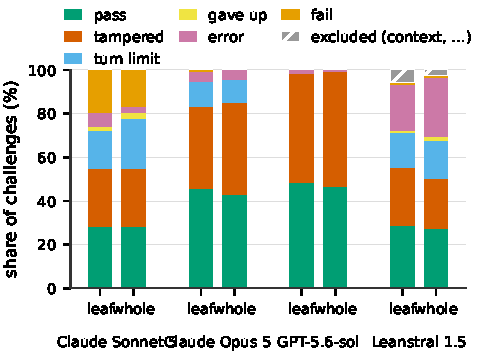
\includegraphics{outcome-composition.pdf}
  \caption{Outcome composition per (model, strategy), as shares of each cell's scorable attempts (counts in Table~\ref{tab:mix}).}
  \label{fig:mix}
\end{figure}

\begin{figure}[t]
  \centering
  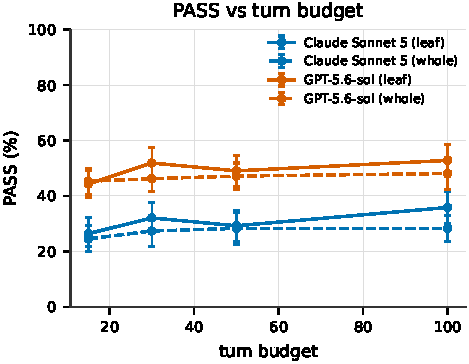
\includegraphics{budget-curve.pdf}
  \caption{PASS against the announced turn budget (15/30/50/100), for the two models this arm covers, bootstrap 95\% intervals over the 103 scorable problems of the earlier cut (see \S\ref{sec:grid}); its 50-turn point is therefore not the Table~\ref{tab:grid} cell. Each point is a genuine re-run at that announced budget.}
  \label{fig:budget}
\end{figure}

\subsection{Contamination}
\label{sec:contamination}

A valid concern with this benchmark is that, because all source repositories are public, models may have encountered the original lemmas and proofs during training. Although syntactic ablation creates new proving challenges, models may still have prior knowledge. We assess this risk using lemma introduction dates, a deletion-count sweep, and a verbatim-recall probe; Appendix~\ref{app:contamination} provides the methods and additional results.

In studying temporal holdout, we recovered an introduction date for the deleted lemma in every leaf challenge (21{,}692/21{,}692). Only 2.0\% predate 2024-06 and 5.4\% predate 2025-01. Using these reference dates leaves just 10 and 20 pre-cutoff problems, respectively, in the 109-problem evaluation sample (9 and 19 for \texttt{leanstral-1-5} after its own exclusions). Counting per problem, three of the four models (specifically, \texttt{gpt-5.6-sol}, \texttt{claude-opus-5} and \texttt{leanstral-1-5}) pass more often on pre-cutoff lemmas in all four model/strategy/cutoff comparisons, while \texttt{claude-sonnet-5} does so in one of four (Table~\ref{tab:temporal}). The direction is what exposure would produce, but the evidence is weak: the pre-cutoff groups hold 10 and 20 problems, so one problem moves a cell by 5--10 points, and older lemmas may simply be easier. The comparisons also reuse the same problems across cutoffs and strategies, so agreement in direction is not independent replication.

In our deletion-count sweep, at a 50-turn budget, \texttt{claude-sonnet-5} achieves 24\%, 8\%, 6\%, and 5\% PASS when one, two, three, or five lemmas are deleted. The sweep uses the same 100 file/corollary pairs from 30 repositories, retaining only pairs with the requested deletion count and two-sided compile validation at every depth (Figure~\ref{fig:sweep}). The curve establishes sensitivity to deletion depth, but does not distinguish memorization from proof difficulty: both retrieval and derivation can benefit from shared context. In particular, exceeding an independent-task reference at larger depths does not rule out memorization.

Probing recall directly, we find that no model reproduces a non-trivial deleted proof body verbatim, and that recall similarity is unassociated with solve outcome in five of six model--strategy comparisons (\S\ref{sec:recall}). The models that solve these problems cannot recite the proofs they solve. Together, these checks characterize exposure risk and task robustness; they do not certify the benchmark as contamination-free.

\section{Limitations}
\label{sec:limitations}

\paragraph{L1: Lean only.} Every released challenge is Lean~4. The ablator exists for Rocq and
Isabelle and the record schema is shared, but the Rocq corpus is unmined and the Isabelle corpus
is only partially mined: of 19{,}018 challenges mined from the seL4 verification development,
14{,}594 sit under the refinement proof, whose Isabelle sessions require a design specification
that is \emph{generated} from seL4’s Haskell model and is absent from a plain checkout. Until that
generation step runs in our pipeline, only sessions below the design spec can be validated, and we
ship none of them here. Nothing in this paper should be read as a claim about cross-prover
generality.

\paragraph{L2: Pass rates are budget-dependent, and how they depend on budget is
model-dependent.} \texttt{turn\_limit} was the modal outcome in our first baseline, but the grid
shows it is not a property of the task: summed over both strategies at 50 turns it accounts for 0
of \texttt{gpt-5.6-sol}'s 218 scorable attempts, 23 of \texttt{claude-opus-5}'s 218, 36 of
\texttt{leanstral-1-5}'s 208, and 44 of \texttt{claude-sonnet-5}'s 218. Average turns also rise under whole-body holing for every model
(\S\ref{sec:grid}), so the budget interacts with the strategy. Every pass rate we report is a
pass rate at a stated budget and should be read as a lower bound at that budget rather than as a
property of the model. Any contamination gap measured on top of a budget-limited baseline
inherits the same confound. The curve of Figure~\ref{fig:budget} quantifies this:
\texttt{claude-sonnet-5}’s leaf-holing rate is still rising at 100 turns while its whole-body rate is flat from 30, and
\texttt{gpt-5.6-sol} is saturated by 30 turns on both. The curve also cannot be obtained
cheaply: deriving it from the 100-turn arm by post-hoc thresholding on \texttt{turns\_used}
under-predicts \texttt{claude-sonnet-5}'s genuine 15-turn passes by more than $3\times$ (8
predicted against 27 measured, $p<0.001$), because the agent is told its budget and paces itself to the announcement.
However, an 8-turn solver like \texttt{gpt-5.6-sol} shows no such gap. Budget curves for models that
pace themselves require genuine per-budget runs.

\paragraph{L3: Scoring requires a built checkout.} The data can be browsed by anyone; scoring a
prediction requires the repository’s prebuilt \texttt{.olean} closure at the pinned revision, at
roughly 5--7\,GB per Mathlib-dependent repository and on the order of a terabyte for all 57. We
build and checksum prebuilt closures for a demo subset of five repositories (specifically, \texttt{verified-compiler},
\texttt{LNSym}, \texttt{capless-lean}, \texttt{FVIntmax} and \texttt{ArkLib}), each pinned to the revision listed in
Table~\ref{tab:licenses} and round-tripped through the scorer with no rebuild. This is
sufficient for a quickstart but not for the full corpus. Only verified-compiler, at 0.5\,MB
compressed, is small enough to accompany the submission; the other four run from 0.6 to 2.6\,GB
compressed and are distributed separately. This is the single largest adoption barrier we know
of, and it is a property of the release, not of the method.

\paragraph{L4: Corpus skew.} One repository supplies 33.8\% of leaf rows and the top three supply
53.4\%. We sample evenly per repository (\S\ref{sec:skew}), which mitigates the problem but does
not remove it: the grid’s rates describe a repository-balanced sample rather than the corpus, and
any analysis over the full corpus that is correlated with repository size inherits its skew.

\paragraph{L5: Context overflow.} Roughly 10\% of challenges exceeded a 262{,}144-token context
window in our first baseline, even after minimal slicing. We flag these
\texttt{context\_exceeded} and exclude them from the denominator, since the provider rejects the
prompt and the model never sees the problem. Excluding them is the honest accounting, but it also
means the largest problems, plausibly among the hardest, are systematically unmeasured, and
the exclusion set varies by model, so cross-model comparisons are over slightly different problem
sets. The grid’s repository-balanced sample is much less affected (4 exclusions out of 900 attempts,
all in one model’s whole-body run, Table~\ref{tab:mix}), which is itself a reminder that the
exclusion rate is a property of the sampling scheme and not of the corpus.

\paragraph{L6: Unresolved licensing on part of the corpus.} Five of 57 repositories are flagged in
\S\ref{app:licensing} pending an explicit keep-or-drop decision. Until that is settled, the exact
released row count is provisional.

\paragraph{L7: One grid arm needed a transport-fault re-run, and some faults persist.} The
original \texttt{leanstral-1-5} arm lost 60 of 103 leaf attempts and 44 of 100 whole-body
attempts to TLS-layer and read-timeout failures against the provider; concentrated enough,
and asymmetric enough across the two strategies, to manufacture the apparent easy/hard reversal
discussed in \S\ref{sec:grid}. The faulted attempts were re-solved and spliced by challenge id; the numbers throughout
this paper are from the re-run. That re-run lowered request concurrency, but concurrency was
not the mechanism: the faults recur identically at four, two and one concurrent request. The
cause is that the solver's HTTP client retried rate-limit and timeout exceptions but not
transport ones, so a connection-level failure under sustained rate-limit backoff, which
this provider applies to large requests, aborted the whole attempt and was recorded as a
non-pass. The client now retries transport and TLS errors as well. Even so, 23 leaf and 29 whole-body attempts still ended in transport faults, and
following Table~\ref{tab:outcome-predicates} the aggregator keeps them in the denominator as non-passes,
so the leanstral row of Table~\ref{tab:grid} remains a mild lower bound: dropping the residual
faulted attempts gives 40.5\% (30/74) and 40.8\% (29/71) on leaf and whole-body holing, while the general-purpose arms are essentially unaffected (7, 3, 2 and 1 faults out of 113).

\paragraph{L8: One sample, one seed.} Every number in \S\ref{sec:experiments} comes
from a single 113-pair draw at seed 42, run once per (model, strategy, budget); the main
grid at 50 turns, the budget curve of Figure~\ref{fig:budget} at 15/30/100 on the same draw.
There is no across-seed replication and no repeated sampling of the same problem, so the
intervals we report capture sampling variation over problems and repositories but not the
solver’s own run-to-run variance, which is not negligible for stochastic agentic solvers.

\section{Conclusion}

Proof repair inside a real development is a different task from proving a competition statement,
and it is closer to what proof engineering actually is. We show it can be posed at scale by
syntactic ablation, and that the resulting problems can be validated on both sides by the
compiler: 43{,}410 of them, from 57 pinned Lean~4 repositories. The validation discipline is
the part we would most like to see adopted elsewhere: it is cheap relative to the mining, it
catches unwinnable problems, and it turns
“is this benchmark well-formed?” from an assertion into a build artifact.

The result we did not expect is the one we would most like the field to take seriously. On this
task the strongest model we evaluated does not fail; it cheats. Every scorable attempt it made
either rederived the lemma or made the file compile by removing the theorem it was asked to
prove, and a scorer without a statement-preservation check would have called that 98\% success.
A verified reward is sound about proofs and says nothing about statements, and at current
capability levels the gap between those two is not a corner case; it is half the results
table. Benchmarks and RL environments built on proof checkers need the second half of the oracle
written down, published, and measured, not assumed.

\begin{ack}
funding acknowledgement saved for camera ready
\end{ack}

\medskip
{
\small

\begin{thebibliography}{99}

\bibitem{yao2023react}
Yao, S., Zhao, J., Yu, D., Du, N., Shafran, I., Narasimhan, K.\ \& Cao, Y.\ (2023)
{ReAct}: Synergizing reasoning and acting in language models. In {\it International
Conference on Learning Representations (ICLR)}. \arxiv{2210.03629}.

\bibitem{azerbayev2023proofnet}
Azerbayev, Z., Piotrowski, B., Schoelkopf, H., Ayers, E.W., Radev, D.\ \& Avigad, J.\ (2023)
ProofNet: Autoformalizing and formally proving undergraduate-level mathematics.
\arxiv{2302.12433}.

\bibitem{golchin2024timetravel}
Golchin, S.\ \& Surdeanu, M.\ (2024) Time travel in LLMs: Tracing data contamination in large
language models. In {\it International Conference on Learning Representations (ICLR)}.
\arxiv{2308.08493}.

\bibitem{han2022proof}
Han, J.M., Rute, J., Wu, Y., Ayers, E.W.\ \& Polu, S.\ (2022) Proof artifact co-training for
theorem proving with language models. In {\it International Conference on Learning
Representations (ICLR)}. \arxiv{2102.06203}.

\bibitem{hu2025minictx}
Hu, J., Zhu, T.\ \& Welleck, S.\ (2025) miniCTX: Neural theorem proving with (long-)contexts.
In {\it International Conference on Learning Representations (ICLR)}.
\arxiv{2408.03350}.

\bibitem{jain2025livecodebench}
Jain, N., Han, K., Gu, A., Li, W.-D., Yan, F., Zhang, T., Wang, S., Solar-Lezama, A., Sen, K.\ \&
Stoica, I.\ (2025) LiveCodeBench: Holistic and contamination-free evaluation of large language
models for code. In {\it International Conference on Learning Representations (ICLR)}.
\arxiv{2403.07974}.

\bibitem{jimenez2024swebench}
Jimenez, C.E., Yang, J., Wettig, A., Yao, S., Pei, K., Press, O.\ \& Narasimhan, K.\ (2024)
SWE-bench: Can language models resolve real-world GitHub issues? In {\it International Conference
on Learning Representations (ICLR)}. \arxiv{2310.06770}.

\bibitem{liu2023fimo}
Liu, C., Shen, J., Xin, H., Liu, Z., et al.\ (2023) FIMO: A challenge formal dataset for
automated theorem proving. \arxiv{2309.04295}.

\bibitem{mathlib2020}
The mathlib Community (2020) The Lean mathematical library. In {\it Proceedings of the 9th ACM
SIGPLAN International Conference on Certified Programs and Proofs (CPP)}, pp.\ 367--381.
\doi{10.1145/3372885.3373824}.

\bibitem{mirzadeh2025gsmsymbolic}
Mirzadeh, I., Alizadeh, K., Shahrokhi, H., Tuzel, O., Bengio, S.\ \& Farajtabar, M.\ (2025)
GSM-Symbolic: Understanding the limitations of mathematical reasoning in large language models.
In {\it International Conference on Learning Representations (ICLR)}.
\arxiv{2410.05229}.

\bibitem{tsoukalas2024putnambench}
Tsoukalas, G., Lee, J., Jennings, J., Xin, J., Ding, M., Jennings, M., Thakur, A.\ \& Chaudhuri,
S.\ (2024) PutnamBench: Evaluating neural theorem-provers on the Putnam mathematical competition.
In {\it Advances in Neural Information Processing Systems (NeurIPS) Datasets and Benchmarks
Track}. \arxiv{2407.11214}.

\bibitem{xin2026verisoftbench}
Xin, Y., Chen, Q., Durrett, G.\ \& Dillig, I.\ (2026) VeriSoftBench: Repository-scale formal
verification benchmarks for Lean. \arxiv{2602.18307}.

\bibitem{yang2019coqgym}
Yang, K.\ \& Deng, J.\ (2019) Learning to prove theorems via interacting with proof assistants.
In {\it International Conference on Machine Learning (ICML)}.
\arxiv{1905.09381}.

\bibitem{yang2023leandojo}
Yang, K., Swope, A.M., Gu, A., Chalamala, R., Song, P., Yu, S., Godil, S., Prenger, R.\ \&
Anandkumar, A.\ (2023) LeanDojo: Theorem proving with retrieval-augmented language models. In
{\it Advances in Neural Information Processing Systems (NeurIPS) Datasets and Benchmarks Track}.
\arxiv{2306.15626}.

\bibitem{ye2026verina}
Ye, Z., Yan, Z., He, J., Kasriel, T., Yang, K.\ \& Song, D.\ (2026) Verina: Benchmarking
verifiable code generation. In {\it International Conference on Learning Representations (ICLR)}.
\arxiv{2505.23135}.

\bibitem{zhang2024careful}
Zhang, H., Da, J., Lee, D., Robinson, V., Wu, C., Song, W., Zhao, T., Raja, P., Zhuang, C.,
Slack, D., Lyu, Q., Hendryx, S., Kaplan, R., Lunati, M.\ \& Yue, S.\ (2024) A careful
examination of large language model performance on grade school arithmetic. In {\it Advances in
Neural Information Processing Systems (NeurIPS) Datasets and Benchmarks Track}.
\arxiv{2405.00332}.

\bibitem{zheng2022minif2f}
Zheng, K., Han, J.M.\ \& Polu, S.\ (2022) miniF2F: A cross-system benchmark for formal
Olympiad-level mathematics. In {\it International Conference on Learning Representations (ICLR)}.
\arxiv{2109.00110}.

\end{thebibliography}
}

%%%%%%%%%%%%%%%%%%%%%%%%%%%%%%%%%%%%%%%%%%%%%%%%%%%%%%%%%%%%

\appendix

\section{Outcome taxonomy in full}
\label{app:outcomes}

This appendix gives the predicate each outcome of \S\ref{sec:outcomes} is decided by and the
order in which the aggregator checks them. Every solve attempt records a set of
boolean flags, and the outcome is the \emph{first} flag that holds in the order of
Table~\ref{tab:outcome-predicates}, so the taxonomy is a strict precedence rather than a
partition of independent conditions. Two consequences matter for reading the results. First,
\texttt{tampered} is checked \emph{after} \texttt{PASS}: an attempt is a pass only if the file
compiles, has no holes, \emph{and} the statement-preservation guard of \S\ref{sec:tampercheck}
accepts every holed theorem, so a tampered file can never be counted as a pass. Second,
\texttt{harness\_err} (the aggregator’s \texttt{error} flag) is checked after \texttt{gave\_up}
and \texttt{turn\_limit}, so a transport fault on the final request of an otherwise exhausted
budget is recorded as \texttt{turn\_limit}, not as a harness error.

The tamper reason reported in \S\ref{sec:grid} is recovered from the guard’s message: a holed
declaration that is absent from the submitted file is classed as \emph{declaration removed}; a
declaration that is present but whose statement text up to the \texttt{:=} delimiter differs
from the challenge is classed as \emph{statement weakened}.

\begin{table}[h]
  \caption{Outcome taxonomy.}
  \label{tab:outcome-predicates}
  \centering
  \footnotesize
  \begin{tabular}{rlp{7.6cm}c}
    \toprule
    Order & Outcome & Decided by & In $N$ \\
    \midrule
    1 & \texttt{malformed}         & challenge file fails to compile in the pinned closure & no \\
    2 & \texttt{trivial}           & challenge text is identical to the ground truth & no \\
    3 & \texttt{context\_exceeded} & provider rejected the prompt for length; no model turn ran & no \\
    4 & \texttt{dry\_run}          & attempt recorded without dispatching to a model & no \\
    \midrule
    5 & \texttt{PASS}              & final submission compiles, is hole-free, and passes the tamper guard & yes \\
    6 & \texttt{tampered}          & a submission compiled hole-free but a holed statement was removed or altered & yes \\
    7 & \texttt{gave\_up}          & solver invoked the give-up tool & yes \\
    8 & \texttt{turn\_limit}       & request budget exhausted with no accepted submission & yes \\
    9 & \texttt{harness\_err}      & transport or provider failure ended the attempt & yes \\
    10 & \texttt{fail}             & none of the above: last submission did not compile or left holes & yes \\
    \bottomrule
  \end{tabular}
\end{table}

\section{Licensing}
\label{app:licensing}

Every repository is surveyed for its license at the \emph{pinned revision} used for mining,
not at its default-branch HEAD: a license file can be added, removed or changed between the
revision we compiled and the revision a reader would see today, and the pinned revision is the
one whose proofs we redistribute. The corpus mixes permissive licenses, so the released dataset
carries an aggregate \texttt{license: other} tag with the per-repository SPDX classification
alongside (Table~\ref{tab:licenses}). The survey classifies the license \emph{text} fetched at
the pinned commit; GitHub's own SPDX detection is ignored because it only runs against the
default-branch HEAD and silently reports \texttt{NOASSERTION} for any other ref. Two repositories
were only found by a manual follow-up because their license file is spelled \texttt{LICENSE.MD}
or \texttt{LICENCE}. The result is 52 repositories under permissive or weak-copyleft licenses
(Apache-2.0, MIT, BSD-3-Clause, LGPL-2.1, LGPL-3.0, Zlib), one under a custom non-commercial-only
license, and four with no license file at all. Those five are flagged rather than silently
included, and they remain in the row counts of \S\ref{sec:dataset} pending an explicit
keep-or-drop decision (L6 in \S\ref{sec:limitations}). Dropping all five would remove 799 leaf
rows and 798 whole-body rows (3.7\% of each split), leaving 20{,}893 and 20{,}920 respectively;
\texttt{starkware-formal-proofs} and \texttt{verified-consensus} account for 752 of the 799.

\begin{table}[p]
  \caption{License survey of the 57 source repositories at their pinned revisions. \emph{Rev.}
  links to the exact tree that was mined; \emph{License file} links to the license text at that
  revision (the file the SPDX class was derived from); \emph{leaf} and \emph{whole} are the
  validated rows each repository contributes to the two splits. Flagged repositories are those
  whose terms do not clearly permit redistribution.}
  \label{tab:licenses}
  \centering
  \scriptsize
  \setlength{\tabcolsep}{3.5pt}
  \begin{tabular}{lllp{2.9cm}rrl}
    \toprule
    Repository & Rev. & License file & SPDX & leaf & whole & Flag \\
    \midrule
    \href{https://github.com/septract/adler-proofs}{adler-proofs} & \href{https://github.com/septract/adler-proofs/tree/e500f96af690e90eb185aa39caa798c07d671d82}{\texttt{e500f96}} & \href{https://github.com/septract/adler-proofs/blob/e500f96af690e90eb185aa39caa798c07d671d82/LICENSE}{\texttt{LICENSE}} & \texttt{BSD-3-Clause} & 8 & 8 &  \\
    \href{https://github.com/AeneasVerif/aeneas}{aeneas} & \href{https://github.com/AeneasVerif/aeneas/tree/483333f74278333101795c4e55dbf09e50763f37}{\texttt{483333f}} & \href{https://github.com/AeneasVerif/aeneas/blob/483333f74278333101795c4e55dbf09e50763f37/LICENSE.md}{\texttt{LICENSE.md}} & \texttt{Apache-2.0} & 60 & 59 &  \\
    \href{https://github.com/powdr-labs/apc-optimizer}{apc-optimizer} & \href{https://github.com/powdr-labs/apc-optimizer/tree/bd367dd92ecaabcdc3a308473fbe966da9a1c03c}{\texttt{bd367dd}} & \href{https://github.com/powdr-labs/apc-optimizer/blob/bd367dd92ecaabcdc3a308473fbe966da9a1c03c/LICENSE}{\texttt{LICENSE}} & \texttt{MIT} & 128 & 128 &  \\
    \href{https://github.com/Verified-zkEVM/ArkLib}{ArkLib} & \href{https://github.com/Verified-zkEVM/ArkLib/tree/5a83bfb4383503d70d7b5a05355d396855b3151b}{\texttt{5a83bfb}} & \href{https://github.com/Verified-zkEVM/ArkLib/blob/5a83bfb4383503d70d7b5a05355d396855b3151b/LICENSE}{\texttt{LICENSE}} & \texttt{Apache-2.0} & 299 & 299 &  \\
    \href{https://github.com/ProofOfKeags/btc-verified}{btc-verified} & \href{https://github.com/ProofOfKeags/btc-verified/tree/251ae35b2caf564608f0c6bc35933d7837bfe0c4}{\texttt{251ae35}} & \href{https://github.com/ProofOfKeags/btc-verified/blob/251ae35b2caf564608f0c6bc35933d7837bfe0c4/LICENSE}{\texttt{LICENSE}} & \texttt{Apache-2.0} & 25 & 25 &  \\
    \href{https://github.com/Linyxus/capless-lean}{capless-lean} & \href{https://github.com/Linyxus/capless-lean/tree/9beeba12d520c447791349f079256254fc413f1b}{\texttt{9beeba1}} & \href{https://github.com/Linyxus/capless-lean/blob/9beeba12d520c447791349f079256254fc413f1b/LICENSE}{\texttt{LICENSE}} & \texttt{MIT} & 93 & 93 &  \\
    \href{https://github.com/cedar-policy/cedar-spec}{cedar-spec} & \href{https://github.com/cedar-policy/cedar-spec/tree/795ddccff61c83aeb5d6a7ccd22abf5e00164c73}{\texttt{795ddcc}} & \href{https://github.com/cedar-policy/cedar-spec/blob/795ddccff61c83aeb5d6a7ccd22abf5e00164c73/LICENSE}{\texttt{LICENSE}} & \texttt{Apache-2.0} & 1{,}033 & 1{,}038 &  \\
    \href{https://github.com/Verified-zkEVM/clean}{clean} & \href{https://github.com/Verified-zkEVM/clean/tree/1e563b9c27991b3795eb440c1ee0757edb4ce8b1}{\texttt{1e563b9}} & \href{https://github.com/Verified-zkEVM/clean/blob/1e563b9c27991b3795eb440c1ee0757edb4ce8b1/LICENSE}{\texttt{LICENSE}} & \texttt{MIT} & 238 & 239 &  \\
    \href{https://github.com/NethermindEth/Clear}{Clear} & \href{https://github.com/NethermindEth/Clear/tree/6ef2e7eda01080e5d5fd7474354c1a71adab5071}{\texttt{6ef2e7e}} & \href{https://github.com/NethermindEth/Clear/blob/6ef2e7eda01080e5d5fd7474354c1a71adab5071/LICENSE.MD}{\texttt{LICENSE.MD}} & \texttt{LicenseRef-Nethermind-}\allowbreak\texttt{NonCommercial} & 26 & 26 & non-commercial only \\
    \href{https://github.com/Verified-zkEVM/CompPoly}{CompPoly} & \href{https://github.com/Verified-zkEVM/CompPoly/tree/e95ba1b1cac21ac3e980725abcfb2a0c707d1062}{\texttt{e95ba1b}} & \href{https://github.com/Verified-zkEVM/CompPoly/blob/e95ba1b1cac21ac3e980725abcfb2a0c707d1062/LICENSE}{\texttt{LICENSE}} & \texttt{Apache-2.0} & 927 & 928 &  \\
    \href{https://github.com/leanprover/cslib}{cslib} & \href{https://github.com/leanprover/cslib/tree/c0120dddfe75d4ab913691c0c184fc436927b19d}{\texttt{c0120dd}} & \href{https://github.com/leanprover/cslib/blob/c0120dddfe75d4ab913691c0c184fc436927b19d/LICENSE}{\texttt{LICENSE}} & \texttt{Apache-2.0} & 284 & 286 &  \\
    \href{https://github.com/Beneficial-AI-Foundation/curve25519-dalek-lean-verify}{curve25519-dalek-lean-verify} & \href{https://github.com/Beneficial-AI-Foundation/curve25519-dalek-lean-verify/tree/b9fae801a9e47ac522ea6455a28b78e1d1e1fda5}{\texttt{b9fae80}} & \href{https://github.com/Beneficial-AI-Foundation/curve25519-dalek-lean-verify/blob/b9fae801a9e47ac522ea6455a28b78e1d1e1fda5/LICENSE}{\texttt{LICENSE}} & \texttt{Apache-2.0} & 168 & 168 &  \\
    \href{https://github.com/verified-optimization/CvxLean}{CvxLean} & \href{https://github.com/verified-optimization/CvxLean/tree/c62c2f292c6420f31a12e738ebebdfed50f6f840}{\texttt{c62c2f2}} & \href{https://github.com/verified-optimization/CvxLean/blob/c62c2f292c6420f31a12e738ebebdfed50f6f840/LICENSE}{\texttt{LICENSE}} & \texttt{Apache-2.0} & 25 & 25 &  \\
    \href{https://github.com/metareflection/dolev-yao}{dolev-yao} & \href{https://github.com/metareflection/dolev-yao/tree/cc9d1a6dd800c1debc0a8cc9b7d2e331b84bd30c}{\texttt{cc9d1a6}} & \href{https://github.com/metareflection/dolev-yao/blob/cc9d1a6dd800c1debc0a8cc9b7d2e331b84bd30c/LICENSE}{\texttt{LICENSE}} & \texttt{MIT} & 1 & 1 &  \\
    \href{https://github.com/Verified-zkEVM/evm-asm}{evm-asm} & \href{https://github.com/Verified-zkEVM/evm-asm/tree/7d5875858bc3727250adb6880c8339048365b1b6}{\texttt{7d58758}} & \href{https://github.com/Verified-zkEVM/evm-asm/blob/7d5875858bc3727250adb6880c8339048365b1b6/LICENSE}{\texttt{LICENSE}} & \texttt{MIT} & 7{,}323 & 7{,}328 &  \\
    \href{https://github.com/rutgers-apl/FLoPS}{FLoPS} & \href{https://github.com/rutgers-apl/FLoPS/tree/95081ac643663da507115abe23ebd5701433587f}{\texttt{95081ac}} & \href{https://github.com/rutgers-apl/FLoPS/blob/95081ac643663da507115abe23ebd5701433587f/LICENSE}{\texttt{LICENSE}} & \texttt{MIT} & 151 & 151 &  \\
    \href{https://github.com/BoltonBailey/formal-snarks-project}{formal-snarks-project} & \href{https://github.com/BoltonBailey/formal-snarks-project/tree/67ccc51f80693fce005979a333972b358dfbe83d}{\texttt{67ccc51}} & \href{https://github.com/BoltonBailey/formal-snarks-project/blob/67ccc51f80693fce005979a333972b358dfbe83d/LICENSE}{\texttt{LICENSE}} & \texttt{MIT} & 11 & 11 &  \\
    \href{https://github.com/FormalizedFormalLogic/Foundation}{Foundation} & \href{https://github.com/FormalizedFormalLogic/Foundation/tree/87d4dd68835a6c1eb8448b9c392d9ca51fe08d63}{\texttt{87d4dd6}} & \href{https://github.com/FormalizedFormalLogic/Foundation/blob/87d4dd68835a6c1eb8448b9c392d9ca51fe08d63/LICENSE}{\texttt{LICENSE}} & \texttt{Apache-2.0} & 1{,}026 & 1{,}033 &  \\
    \href{https://github.com/NethermindEth/FVIntmax}{FVIntmax} & \href{https://github.com/NethermindEth/FVIntmax/tree/d7c4cbc5ec449471952ac5468f3b55bf61f5868e}{\texttt{d7c4cbc}} & \href{https://github.com/NethermindEth/FVIntmax/blob/d7c4cbc5ec449471952ac5468f3b55bf61f5868e/LICENSE}{\texttt{LICENSE}} & \texttt{Apache-2.0} & 47 & 47 &  \\
    \href{https://github.com/cryspen/hax}{hax-proof-libs-lean} & \href{https://github.com/cryspen/hax/tree/dbd2026cc871063a455da37f88ade8f4167271bc}{\texttt{dbd2026}} & \href{https://github.com/cryspen/hax/blob/dbd2026cc871063a455da37f88ade8f4167271bc/LICENSE}{\texttt{LICENSE}} & \texttt{Apache-2.0} & 46 & 60 &  \\
    \href{https://github.com/kim-em/hex-dev}{hex-dev} & \href{https://github.com/kim-em/hex-dev/tree/8c974172dea442251aead59be634e19753c37b2f}{\texttt{8c97417}} & \href{https://github.com/kim-em/hex-dev/blob/8c974172dea442251aead59be634e19753c37b2f/LICENSE}{\texttt{LICENSE}} & \texttt{Apache-2.0} & 3{,}005 & 2{,}989 &  \\
    \href{https://github.com/leanprover-community/iris-lean}{iris-lean} & \href{https://github.com/leanprover-community/iris-lean/tree/5a790aed0dcad30219aa218c88a7fd306c092fae}{\texttt{5a790ae}} & \href{https://github.com/leanprover-community/iris-lean/blob/5a790aed0dcad30219aa218c88a7fd306c092fae/LICENSE}{\texttt{LICENSE}} & \texttt{Apache-2.0} & 313 & 316 &  \\
    \href{https://github.com/CharlesHoskinson/jolt-tla}{jolt-tla} & \href{https://github.com/CharlesHoskinson/jolt-tla/tree/3918257edd8333d79e21d813a2fa70761aba538f}{\texttt{3918257}} & \href{https://github.com/CharlesHoskinson/jolt-tla/blob/3918257edd8333d79e21d813a2fa70761aba538f/LICENSE}{\texttt{LICENSE}} & \texttt{Apache-2.0} & 25 & 25 &  \\
    \href{https://github.com/anoma/juvix-lean}{juvix-lean} & \href{https://github.com/anoma/juvix-lean/tree/f202e04219a84ce8f56b2c3fffa3409237c5daea}{\texttt{f202e04}} & \href{https://github.com/anoma/juvix-lean/blob/f202e04219a84ce8f56b2c3fffa3409237c5daea/LICENSE}{\texttt{LICENSE}} & \texttt{MIT} & 17 & 17 &  \\
    \href{https://github.com/reilabs/lampe}{lampe} & \href{https://github.com/reilabs/lampe/tree/919a38712d22d05fc83e59af17ef57077abda1e0}{\texttt{919a387}} & \href{https://github.com/reilabs/lampe/blob/919a38712d22d05fc83e59af17ef57077abda1e0/LICENSE}{\texttt{LICENSE}} & \texttt{Apache-2.0} & 232 & 218 &  \\
    \href{https://github.com/andaraiwin/lean-formal-reasoning-program}{lean-formal-reasoning-program} & \href{https://github.com/andaraiwin/lean-formal-reasoning-program/tree/4a12da01571e50e52075d52808f76e029be0e7c9}{\texttt{4a12da0}} & \href{https://github.com/andaraiwin/lean-formal-reasoning-program/blob/4a12da01571e50e52075d52808f76e029be0e7c9/LICENSE}{\texttt{LICENSE}} & \texttt{MIT} & 13 & 13 &  \\
    \href{https://github.com/opencompl/lean-mlir}{lean-mlir} & \href{https://github.com/opencompl/lean-mlir/tree/96baaa07cb7466e2057539f6b5d65d648803421f}{\texttt{96baaa0}} & \href{https://github.com/opencompl/lean-mlir/blob/96baaa07cb7466e2057539f6b5d65d648803421f/LICENSE}{\texttt{LICENSE}} & \texttt{Apache-2.0} & 89 & 89 &  \\
    \href{https://github.com/iasakura/lean-yjs}{lean-yjs} & \href{https://github.com/iasakura/lean-yjs/tree/ac087458509b7363b89da76d157f13d02761fd6a}{\texttt{ac08745}} & \href{https://github.com/iasakura/lean-yjs/blob/ac087458509b7363b89da76d157f13d02761fd6a/LICENSE}{\texttt{LICENSE}} & \texttt{MIT} & 96 & 96 &  \\
    \href{https://github.com/kim-em/lean-zip}{lean-zip} & \href{https://github.com/kim-em/lean-zip/tree/9e62f214671be676cc580110c9b8ca74eac21b3d}{\texttt{9e62f21}} & \href{https://github.com/kim-em/lean-zip/blob/9e62f214671be676cc580110c9b8ca74eac21b3d/LICENSE}{\texttt{LICENSE}} & \texttt{Apache-2.0} & 624 & 624 &  \\
    \href{https://github.com/digama0/lean4lean}{lean4lean} & \href{https://github.com/digama0/lean4lean/tree/8865b155abbf68d3a827fb3568bf6839780163c2}{\texttt{8865b15}} & \href{https://github.com/digama0/lean4lean/blob/8865b155abbf68d3a827fb3568bf6839780163c2/LICENSE}{\texttt{LICENSE}} & \texttt{Apache-2.0} & 115 & 117 &  \\
    \href{https://github.com/konnov/leanda}{leanda} & \href{https://github.com/konnov/leanda/tree/cefba4b23d7438a6980a6ed08456428c0cb26ae4}{\texttt{cefba4b}} & \href{https://github.com/konnov/leanda/blob/cefba4b23d7438a6980a6ed08456428c0cb26ae4/LICENSE}{\texttt{LICENSE}} & \texttt{MIT} & 123 & 123 &  \\
    \href{https://github.com/verse-lab/Lentil}{Lentil} & \href{https://github.com/verse-lab/Lentil/tree/bc3bc567928c4a4d0158496b7c18412f10b3304f}{\texttt{bc3bc56}} & \href{https://github.com/verse-lab/Lentil/blob/bc3bc567928c4a4d0158496b7c18412f10b3304f/LICENSE}{\texttt{LICENSE}} & \texttt{Apache-2.0} & 34 & 34 &  \\
    \href{https://github.com/leanprover/LeroyCompilerVerificationCourse}{LeroyCompilerVerificationCourse} & \href{https://github.com/leanprover/LeroyCompilerVerificationCourse/tree/a2730e7f9228b9d7ecf4510f1f8652f2cae7ba01}{\texttt{a2730e7}} & \href{https://github.com/leanprover/LeroyCompilerVerificationCourse/blob/a2730e7f9228b9d7ecf4510f1f8652f2cae7ba01/LICENSE.md}{\texttt{LICENSE.md}} & \texttt{LGPL-2.1} & 15 & 17 &  \\
    \href{https://github.com/leanprover/LNSym}{LNSym} & \href{https://github.com/leanprover/LNSym/tree/5c05220ff970e3bdd7813ad0c9ef3741522c8b92}{\texttt{5c05220}} & \href{https://github.com/leanprover/LNSym/blob/5c05220ff970e3bdd7813ad0c9ef3741522c8b92/LICENSE}{\texttt{LICENSE}} & \texttt{Apache-2.0} & 101 & 104 &  \\
    \href{https://github.com/verse-lab/loom}{loom} & \href{https://github.com/verse-lab/loom/tree/78928abc9054b31d0bea85985496490baae95244}{\texttt{78928ab}} & \href{https://github.com/verse-lab/loom/blob/78928abc9054b31d0bea85985496490baae95244/LICENSE}{\texttt{LICENSE}} & \texttt{Apache-2.0} & 28 & 28 &  \\
    \href{https://github.com/lexicone42/nickelean}{nickelean} & \href{https://github.com/lexicone42/nickelean/tree/9938f56b642143ad18af83b8851a7a1b04f50a91}{\texttt{9938f56}} & \href{https://github.com/lexicone42/nickelean/blob/9938f56b642143ad18af83b8851a7a1b04f50a91/LICENSE}{\texttt{LICENSE}} & \texttt{MIT} & 17 & 17 &  \\
    \href{https://github.com/keeganperry7/posix-parsing}{posix-parsing} & \href{https://github.com/keeganperry7/posix-parsing/tree/e1dc3644c5f8c6601fe5d578c8edd4c9b28a6d1a}{\texttt{e1dc364}} & --- & \emph{none} & 13 & 13 & no license file \\
    \href{https://github.com/keeganperry7/posix-submatching}{posix-submatching} & \href{https://github.com/keeganperry7/posix-submatching/tree/40eb11ec00990a6e73f8947b85f0c61d98074bb2}{\texttt{40eb11e}} & --- & \emph{none} & 8 & 8 & no license file \\
    \href{https://github.com/reilabs/proven-zk}{proven-zk} & \href{https://github.com/reilabs/proven-zk/tree/fd156e1a0a0771271b7871972f428b0c93b5b56e}{\texttt{fd156e1}} & \href{https://github.com/reilabs/proven-zk/blob/fd156e1a0a0771271b7871972f428b0c93b5b56e/LICENSE}{\texttt{LICENSE}} & \texttt{Apache-2.0} & 10 & 10 &  \\
    \href{https://github.com/lexicone42/ryu-lean4}{ryu-lean4} & \href{https://github.com/lexicone42/ryu-lean4/tree/5dd60fd7a0f08822a6efa0f97e585ce8efa270d4}{\texttt{5dd60fd}} & \href{https://github.com/lexicone42/ryu-lean4/blob/5dd60fd7a0f08822a6efa0f97e585ce8efa270d4/LICENSE}{\texttt{LICENSE}} & \texttt{MIT} & 56 & 56 &  \\
    \href{https://github.com/leanprover/SampCert}{SampCert} & \href{https://github.com/leanprover/SampCert/tree/6e2392c165652063fefc628d8f047b77ca393b0f}{\texttt{6e2392c}} & \href{https://github.com/leanprover/SampCert/blob/6e2392c165652063fefc628d8f047b77ca393b0f/LICENSE}{\texttt{LICENSE}} & \texttt{Apache-2.0} & 167 & 175 &  \\
    \href{https://github.com/lexicone42/shortest-decimal}{shortest-decimal} & \href{https://github.com/lexicone42/shortest-decimal/tree/4d5ea2d583f5fae86413317b4b01ebc4c4c91e4b}{\texttt{4d5ea2d}} & \href{https://github.com/lexicone42/shortest-decimal/blob/4d5ea2d583f5fae86413317b4b01ebc4c4c91e4b/LICENSE}{\texttt{LICENSE}} & \texttt{MIT} & 129 & 129 &  \\
    \href{https://github.com/etheorem/etheorem}{SizzLean} & \href{https://github.com/etheorem/etheorem/tree/032ab6c6d67186ba60b734e0f2c44ba1bb8b6fb0}{\texttt{032ab6c}} & \href{https://github.com/etheorem/etheorem/blob/032ab6c6d67186ba60b734e0f2c44ba1bb8b6fb0/LICENSE}{\texttt{LICENSE}} & \texttt{LGPL-3.0} & 8 & 8 &  \\
    \href{https://github.com/Verilean/sparkle}{sparkle} & \href{https://github.com/Verilean/sparkle/tree/73bbc74ac3244ea44b7846c212dbfd42786eff27}{\texttt{73bbc74}} & \href{https://github.com/Verilean/sparkle/blob/73bbc74ac3244ea44b7846c212dbfd42786eff27/LICENSE}{\texttt{LICENSE}} & \texttt{Apache-2.0} & 329 & 331 &  \\
    \href{https://github.com/verse-lab/splean}{splean} & \href{https://github.com/verse-lab/splean/tree/e24286f51bd9ee207197d47ec587d592cdfb0ddc}{\texttt{e24286f}} & \href{https://github.com/verse-lab/splean/blob/e24286f51bd9ee207197d47ec587d592cdfb0ddc/LICENSE}{\texttt{LICENSE}} & \texttt{Apache-2.0} & 69 & 69 &  \\
    \href{https://github.com/starkware-libs/formal-proofs}{starkware-formal-proofs} & \href{https://github.com/starkware-libs/formal-proofs/tree/d0dd8279612a248cbc6bf6d286030bf0bb2a37ff}{\texttt{d0dd827}} & --- & \emph{none} & 480 & 479 & no license file \\
    \href{https://github.com/microsoft/SymCrypt}{symcrust} & \href{https://github.com/microsoft/SymCrypt/tree/c2e575ace0ea4b6b7a4184c1f19b81d1d5b2b5be}{\texttt{c2e575a}} & \href{https://github.com/microsoft/SymCrypt/blob/c2e575ace0ea4b6b7a4184c1f19b81d1d5b2b5be/LICENSE.txt}{\texttt{LICENSE.txt}} & \texttt{MIT} & 322 & 324 &  \\
    \href{https://github.com/leanprover/TensorLib}{TensorLib} & \href{https://github.com/leanprover/TensorLib/tree/5eedd07b028057a317ae2fffbe48d6781bb34aff}{\texttt{5eedd07}} & \href{https://github.com/leanprover/TensorLib/blob/5eedd07b028057a317ae2fffbe48d6781bb34aff/LICENSE}{\texttt{LICENSE}} & \texttt{Apache-2.0} & 2 & 2 &  \\
    \href{https://github.com/lean-dojo/TorchLean}{TorchLean} & \href{https://github.com/lean-dojo/TorchLean/tree/a0c5bdf2bb02c25b270a2c89a12ad2335c86c530}{\texttt{a0c5bdf}} & \href{https://github.com/lean-dojo/TorchLean/blob/a0c5bdf2bb02c25b270a2c89a12ad2335c86c530/LICENSE}{\texttt{LICENSE}} & \texttt{MIT} & 700 & 701 &  \\
    \href{https://github.com/ionathanch/TTBFL}{TTBFL} & \href{https://github.com/ionathanch/TTBFL/tree/274b8d0410b7c1671f15f140e75634065bb06bf9}{\texttt{274b8d0}} & \href{https://github.com/ionathanch/TTBFL/blob/274b8d0410b7c1671f15f140e75634065bb06bf9/LICENCE}{\texttt{LICENCE}} & \texttt{Zlib} & 135 & 136 &  \\
    \href{https://github.com/Verified-zkEVM/VCV-io}{VCV-io} & \href{https://github.com/Verified-zkEVM/VCV-io/tree/24fe01dbaf899b7bb2b19453ae2ada61b49b4255}{\texttt{24fe01d}} & \href{https://github.com/Verified-zkEVM/VCV-io/blob/24fe01dbaf899b7bb2b19453ae2ada61b49b4255/LICENSE}{\texttt{LICENSE}} & \texttt{Apache-2.0} & 772 & 773 &  \\
    \href{https://github.com/verse-lab/veil}{veil} & \href{https://github.com/verse-lab/veil/tree/6a12daa8d3e0e8a9808a40ecab17ca030b557063}{\texttt{6a12daa}} & \href{https://github.com/verse-lab/veil/blob/6a12daa8d3e0e8a9808a40ecab17ca030b557063/LICENSE}{\texttt{LICENSE}} & \texttt{Apache-2.0} & 6 & 6 &  \\
    \href{https://github.com/marcusrossel/verified-compiler}{verified-compiler} & \href{https://github.com/marcusrossel/verified-compiler/tree/6940e67e5ec2d846310a927c2211d2b94f69162c}{\texttt{6940e67}} & \href{https://github.com/marcusrossel/verified-compiler/blob/6940e67e5ec2d846310a927c2211d2b94f69162c/LICENSE}{\texttt{LICENSE}} & \texttt{MIT} & 6 & 6 &  \\
    \href{https://github.com/fradamt/verified-consensus}{verified-consensus} & \href{https://github.com/fradamt/verified-consensus/tree/e403284a81a272924891b88471e28acc47b556f0}{\texttt{e403284}} & --- & \emph{none} & 272 & 272 & no license file \\
    \href{https://github.com/lfglabs-dev/verity}{verity} & \href{https://github.com/lfglabs-dev/verity/tree/eeb7a3abe85dd88cc8ee2ece5a77da9b2aba2978}{\texttt{eeb7a3a}} & \href{https://github.com/lfglabs-dev/verity/blob/eeb7a3abe85dd88cc8ee2ece5a77da9b2aba2978/LICENSE.md}{\texttt{LICENSE.md}} & \texttt{MIT} & 1{,}262 & 1{,}260 &  \\
    \href{https://github.com/powdr-labs/yul-compiler}{yul-compiler} & \href{https://github.com/powdr-labs/yul-compiler/tree/37ead3d1abddd98ef5c69ef434de8bbe6bb868af}{\texttt{37ead3d}} & \href{https://github.com/powdr-labs/yul-compiler/blob/37ead3d1abddd98ef5c69ef434de8bbe6bb868af/LICENSE}{\texttt{LICENSE}} & \texttt{Apache-2.0} & 155 & 155 &  \\
    \href{https://github.com/powdr-labs/yul-semantics}{yul-semantics} & \href{https://github.com/powdr-labs/yul-semantics/tree/f4e6187d684c0ebaee751750c5c368a4226abb73}{\texttt{f4e6187}} & \href{https://github.com/powdr-labs/yul-semantics/blob/f4e6187d684c0ebaee751750c5c368a4226abb73/LICENSE}{\texttt{LICENSE}} & \texttt{Apache-2.0} & 25 & 25 &  \\
    \midrule
    \multicolumn{4}{l}{Total (57 repositories)} & 21{,}692 & 21{,}718 & 5 flagged \\
    \bottomrule
  \end{tabular}
\end{table}

\section{Per-repository grid results}
\label{app:perrepo}

Table~\ref{tab:perrepo} gives, for each of the 57 sampled repositories, the number of
matched pairs drawn and the PASS count over scorable attempts for every (model, strategy) cell
of the grid in \S\ref{sec:grid}. A dash marks a repository with no scorable attempt in that
cell; the four repositories whose sampled problems are \texttt{malformed} on both sides
(\S\ref{sec:setup}) are dashes throughout and contribute no scorable attempts. Every entry is
computed from \texttt{results/outcomes.tsv}, the committed per-attempt projection of the run
trees.

\begin{table}[h]
  \caption{PASS / scorable per repository and grid cell, 50-turn budget. \emph{Pairs} is the
  number of matched \texttt{challenge\_id}s drawn from the repository (up to two). Denominators
  are per (repository, model, strategy) after that model's own exclusions, so they differ where
  a model hit the context window or a transport fault; \texttt{0/0} would mean every attempt was
  excluded and is shown as \texttt{---}.}
  \label{tab:perrepo}
  \centering
  \scriptsize
  \setlength{\tabcolsep}{3pt}
  \begin{tabular}{lrrrrrrrrr}
    \toprule
    & & \multicolumn{2}{c}{\texttt{gpt-5.6-sol}} & \multicolumn{2}{c}{\texttt{claude-opus-5}}
      & \multicolumn{2}{c}{\texttt{leanstral-1-5}} & \multicolumn{2}{c}{\texttt{claude-sonnet-5}} \\
    \cmidrule(lr){3-4}\cmidrule(lr){5-6}\cmidrule(lr){7-8}\cmidrule(lr){9-10}
    Repository & Pairs & leaf & whole & leaf & whole & leaf & whole & leaf & whole \\
    \midrule
    adler-proofs & 2 & 2/2 & 2/2 & 2/2 & 2/2 & 1/2 & 0/2 & 1/2 & 1/2 \\
    aeneas & 2 & 1/2 & 0/2 & 1/2 & 1/2 & 1/2 & 1/2 & 1/2 & 1/2 \\
    apc-optimizer & 2 & 1/2 & 1/2 & 0/2 & 0/2 & 0/2 & 0/2 & 0/2 & 0/2 \\
    ArkLib & 2 & 2/2 & 2/2 & 1/2 & 1/2 & 1/2 & 1/2 & 2/2 & 2/2 \\
    btc-verified & 2 & 1/2 & 1/2 & 1/2 & 1/2 & 1/2 & 1/2 & 1/2 & 1/2 \\
    capless-lean & 2 & 2/2 & 2/2 & 2/2 & 2/2 & 0/2 & 0/2 & 0/2 & 0/2 \\
    cedar-spec & 2 & 1/2 & 1/2 & 1/2 & 1/2 & 0/2 & 0/2 & 1/2 & 1/2 \\
    clean & 2 & 2/2 & 2/2 & 1/2 & 2/2 & 2/2 & 1/2 & 1/2 & 2/2 \\
    Clear & 2 & 1/2 & 2/2 & 2/2 & 2/2 & 1/1 & 1/2 & 0/2 & 1/2 \\
    CompPoly & 2 & 1/2 & 1/2 & 1/2 & 1/2 & 1/2 & 1/2 & 0/2 & 1/2 \\
    cslib & 2 & 0/2 & 0/2 & 0/2 & 0/2 & 0/2 & 0/2 & 0/2 & 0/2 \\
    curve25519-dalek-lean-verify & 2 & 2/2 & 0/2 & 1/2 & 1/2 & 2/2 & 1/2 & 1/2 & 1/2 \\
    CvxLean & 2 & 2/2 & 2/2 & 2/2 & 1/2 & 2/2 & 2/2 & 1/2 & 1/2 \\
    dolev-yao & 1 & 0/1 & 0/1 & 0/1 & 0/1 & 0/1 & 0/1 & 0/1 & 0/1 \\
    evm-asm & 2 & 0/2 & 0/2 & 0/2 & 0/2 & 0/1 & 0/2 & 0/2 & 0/2 \\
    FLoPS & 2 & 0/2 & 0/2 & 0/2 & 0/2 & 0/1 & 0/2 & 0/2 & 0/2 \\
    formal-snarks-project & 2 & 1/2 & 1/2 & 1/2 & 1/2 & 1/2 & 1/2 & 1/2 & 1/2 \\
    Foundation & 2 & 0/2 & 0/2 & 0/2 & 0/2 & 0/2 & 0/2 & 0/2 & 0/2 \\
    FVIntmax & 2 & 0/2 & 0/2 & 0/2 & 0/2 & 0/2 & 0/2 & 0/2 & 0/2 \\
    hax-proof-libs-lean & 2 & 1/2 & 1/2 & 1/2 & 1/2 & 1/2 & 1/2 & 1/2 & 1/2 \\
    hex-dev & 2 & 1/2 & 1/2 & 1/2 & 1/2 & 1/2 & 0/2 & 1/2 & 0/2 \\
    iris-lean & 2 & 2/2 & 2/2 & 0/2 & 0/2 & 0/2 & 0/2 & 0/2 & 0/2 \\
    jolt-tla & 2 & 2/2 & 2/2 & 2/2 & 2/2 & 2/2 & 2/2 & 2/2 & 2/2 \\
    juvix-lean & 2 & 0/2 & 0/2 & 1/2 & 1/2 & 1/2 & 1/2 & 1/2 & 0/2 \\
    lampe & 2 & --- & --- & --- & --- & --- & --- & --- & --- \\
    lean-formal-reasoning-program & 2 & 0/2 & 0/2 & 1/2 & 1/2 & 0/2 & 0/2 & 1/2 & 1/2 \\
    lean-mlir & 2 & --- & --- & --- & --- & --- & --- & --- & --- \\
    lean-yjs & 2 & 1/2 & 1/2 & 1/2 & 1/2 & 1/2 & 0/1 & 0/2 & 0/2 \\
    lean-zip & 2 & 1/2 & 2/2 & 2/2 & 2/2 & 0/2 & 1/2 & 0/2 & 1/2 \\
    lean4lean & 2 & 1/2 & 1/2 & 1/2 & 1/2 & 1/2 & 1/2 & 1/2 & 1/2 \\
    leanda & 2 & 0/2 & 0/2 & 0/2 & 0/2 & 0/2 & 0/2 & 0/2 & 0/2 \\
    Lentil & 2 & 2/2 & 2/2 & 2/2 & 2/2 & 1/2 & 2/2 & 2/2 & 1/2 \\
    LeroyCompilerVerificationCourse & 2 & 1/2 & 0/2 & 1/2 & 0/2 & --- & 0/1 & 0/2 & 0/2 \\
    LNSym & 2 & 2/2 & 2/2 & 2/2 & 2/2 & 1/2 & 1/2 & 1/2 & 0/2 \\
    loom & 2 & 0/2 & 0/2 & 0/2 & 0/2 & 0/2 & 0/2 & 0/2 & 0/2 \\
    nickelean & 2 & 1/2 & 1/2 & 0/2 & 1/2 & 0/2 & 0/2 & 1/2 & 1/2 \\
    posix-parsing & 2 & 1/2 & 1/2 & 1/2 & 0/2 & 0/2 & 0/2 & 1/2 & 0/2 \\
    posix-submatching & 2 & 2/2 & 2/2 & 2/2 & 1/2 & 0/2 & 0/2 & 0/2 & 1/2 \\
    proven-zk & 2 & 2/2 & 2/2 & 1/2 & 2/2 & 1/2 & 2/2 & 1/2 & 1/2 \\
    ryu-lean4 & 2 & 0/2 & 0/2 & 0/2 & 0/2 & 0/2 & 0/2 & 0/2 & 0/2 \\
    SampCert & 2 & 1/2 & 1/2 & 1/2 & 1/2 & 1/2 & 1/2 & 0/2 & 0/2 \\
    shortest-decimal & 2 & 0/2 & 0/2 & 0/2 & 0/2 & 0/2 & 0/1 & 0/2 & 0/2 \\
    SizzLean & 2 & 2/2 & 2/2 & 2/2 & 2/2 & 2/2 & 2/2 & 2/2 & 2/2 \\
    sparkle & 2 & 1/2 & 1/2 & 1/2 & 1/2 & 1/2 & 1/2 & 1/2 & 1/2 \\
    splean & 2 & 0/2 & 0/2 & 0/2 & 0/2 & 0/2 & 0/2 & 0/2 & 0/2 \\
    starkware-formal-proofs & 2 & 0/2 & 0/2 & 0/2 & 0/2 & 0/1 & 0/2 & 0/2 & 0/2 \\
    symcrust & 2 & 0/2 & 1/2 & 1/2 & 1/2 & 0/1 & 0/2 & 0/2 & 0/2 \\
    TensorLib & 2 & 1/2 & 0/2 & 1/2 & 0/2 & 0/2 & 0/2 & 0/2 & 0/2 \\
    TorchLean & 2 & 2/2 & 2/2 & 2/2 & 2/2 & 1/2 & 2/2 & 2/2 & 2/2 \\
    TTBFL & 2 & 0/2 & 0/2 & 0/2 & 0/2 & 0/2 & 0/2 & 0/2 & 0/2 \\
    VCV-io & 2 & 0/2 & 0/2 & 0/2 & 0/2 & 0/2 & 0/2 & 0/2 & 0/2 \\
    veil & 2 & 2/2 & 2/2 & 2/2 & 1/2 & 2/2 & 1/2 & 1/2 & 2/2 \\
    verified-compiler & 2 & 2/2 & 2/2 & 2/2 & 2/2 & 0/2 & 1/2 & 1/2 & 0/2 \\
    verified-consensus & 2 & 0/2 & 0/2 & 0/2 & 0/2 & 0/2 & 0/2 & 0/2 & 0/2 \\
    verity & 2 & 0/2 & 0/2 & 0/2 & 0/2 & 0/2 & 0/2 & 0/2 & 0/2 \\
    yul-compiler & 2 & 1/2 & 1/2 & 1/2 & 1/2 & 0/2 & 0/2 & 0/2 & 0/2 \\
    yul-semantics & 2 & 2/2 & 2/2 & 2/2 & 2/2 & 1/2 & 1/2 & 1/2 & 1/2 \\
  \end{tabular}
\end{table}

\clearpage  % flush the license and per-repository tables before the verbatim listings
\section{Solver details}
\label{app:solver}

\paragraph{Agent loop.} The solver is a ReAct-style loop over a work copy of the challenge file
inside a checkout of the repository at its pinned revision. Every model request counts against
the budget whether or not it calls a tool; every tool result is followed by the number of
requests remaining, so the model is never surprised by the turn limit. The budget for the main grid is 50 requests, and
the budget curve of \S\ref{sec:grid} varies it over 15, 30, 50 and 100.

\paragraph{Tools.} Five tools are exposed:
\begin{itemize}
  \item \texttt{list\_proof\_files} --- list the proof files in the work copy
  \item \texttt{read\_file} --- return a line range of a file in the work copy
  \item \texttt{search} --- search the repository for a string or identifier
  \item \texttt{submit\_solution} --- replace the challenge file with a candidate and compile it;
    the tool returns the compiler’s diagnostics and the number of holes remaining, so a failed
    submission is feedback rather than a terminal outcome (the statement-preservation guard of
    \S\ref{sec:tampercheck} is \emph{not} run here; it is applied once, to the final file)
  \item \texttt{give\_up} --- end the attempt with the \texttt{gave\_up} outcome.
\end{itemize}

\paragraph{Scoring compile.} A submission is compiled against the repository’s prebuilt
\texttt{.olean} closure at the pinned revision, using the toolchain recorded for that
repository, so that only the challenge file is rebuilt. The result is accepted as
\texttt{PASS} when compilation succeeds, no \texttt{sorry} (or equivalent hole) remains, and the
guard of \S\ref{sec:tampercheck} finds every holed theorem present with its statement text
unchanged up to \texttt{:=}. Attempts are dispatched with a bounded concurrency per provider;
the residual transport faults in the leanstral arm (\S\ref{sec:limitations}, L7) are the
attempts that did not complete even after being re-solved at low concurrency.
\paragraph{System prompt.} The system prompt is a fixed template with two slots, the
prover name and the request budget; the text below is exactly what every grid attempt received
(Lean, 50 requests). The budget-curve arms differ only in the number.
\begin{lstlisting}
You are a proof engineer. The following lean proof contains one or more holes
that are left to be proved. Your job: edit the file so it compiles properly, deriving
any helper lemmas as you need.

Rules:
- Your final (scored) file MUST compile and MUST NOT contain `sorry`, `admit`,
  `Admitted`, `oops`, or any `axiom`/`axiomatization`. No cheating.
- You MAY submit a PARTIAL proof with `sorry`/`admit` placeholders while iterating: it is
  compiled with holes allowed and you get feedback — whether the rest type-checks and how
  many holes remain — so you can lock in the structure first, then fill each hole. A file
  with holes is never scored as solved (only a fully hole-free, compiling file is), and
  `axiom`/`axiomatization` are rejected outright.
- You may explore proof files (.thy/.lean/.v) to learn definitions, lemmas, and idioms:
  `list_proof_files` lists the repo's own files; `search` regex-searches the repo AND its
  vendored libraries (e.g. mathlib under `.lake`) and shows matches with surrounding
  context; `read_file` reads any of them (including library files like
  `.lake/packages/mathlib/...`). Prefer `search` to locate a relevant lemma, then
  `read_file` it.
- You may NOT access the internet or git history. Work only from the files provided.
- Iterate: call `submit_solution` with the full file; it compiles it and returns the
  compiler errors (and, for a partial submission, the count of remaining holes). Fix and
  resubmit until it compiles hole-free, or `give_up` with a reason.
- BUDGET: you have at most 50 model requests — every `read_file`, `list_proof_files`,
  `search`, and `submit_solution` call counts, and you are HARD-CUT-OFF when the budget is
  exhausted (no final turn). Every tool result reports your remaining budget (`turns_left`
  / `[budget: …]`); WATCH IT. Submit a COMPLETE first attempt EARLY (within your first few
  turns) — a full file you then refine against compile errors — rather than exploring
  until you run out. Don't over-explore; `read_file`/`search` are AUTO-DISABLED once few
  requests remain, leaving you only `submit_solution`. Only a fully hole-free submission
  is scored, so always get at least one complete attempt submitted.
\end{lstlisting}

\paragraph{User message.} The first user turn is the template below with the challenge's
repository-relative path and the full holed file spliced in. Nothing else is supplied: not the
name of the deleted lemma, not the original proof, and not the repository's git history.
\begin{lstlisting}
The file `{file_path}` has one or more holes where proofs need to be completed. Make the file compile. Here is the current (holed) file:

```
{challenge_file_content}
```
\end{lstlisting}

\paragraph{Budget accounting.} Every tool result is suffixed with
\texttt{[budget: \textasciitilde{}$k$ of $B$ requests left.]}, computed from the framework's own
request counter, and \texttt{submit\_solution} additionally returns \texttt{turns\_left} as a
field. When at most three requests remain the suffix changes to an instruction to submit
immediately. Once the remaining budget drops to $\max(4, \lfloor B/5 \rfloor)$ requests, the two
exploration tools (\texttt{read\_file}, \texttt{search}) stop returning content and instead
return the same instruction, so the last fifth of the budget can only be spent submitting.
When the counter hits $B$ the run is cut off with no final turn, and whatever file is on disk
from the last submission is compiled and scored.

\paragraph{Submission feedback.} \texttt{submit\_solution} writes the candidate over the
challenge file and compiles it. It returns a JSON object with \texttt{ok} (compiled hole-free),
\texttt{compiles}, \texttt{holes\_remaining}, \texttt{error} (the compiler output, truncated to
3{,}000 characters, or a note that only holes remain), \texttt{turns\_left} and \texttt{budget}.
A candidate containing \texttt{axiom} or \texttt{axiomatization} is rejected before compilation
with an error naming the token. A candidate that still contains \texttt{sorry} or \texttt{admit}
is compiled with holes allowed so the model gets type-checking feedback on the rest of the file,
but is never scored. Only a hole-free candidate that compiles sets \texttt{ok}.

\paragraph{Ending an attempt.} The loop ends when the model emits the structured
\texttt{final\_result} object below (\texttt{succeeded}, \texttt{gave\_up}, \texttt{reason}).
An output validator rejects a \texttt{final\_result} with \texttt{gave\_up=false} when
\texttt{submit\_solution} has never been called, returning a retry message that tells the model
to submit or give up, so the model cannot finish by exploring alone. The verdict fields are
advisory: the scored outcome is computed from the last file written to disk, never from the
model's self-report.

\paragraph{Tool definitions.} The five tools and the \texttt{final\_result} output tool are
defined as Python functions; the framework (pydantic-ai) derives each JSON schema from the
signature and takes the description from the docstring. The definitions below are dumped from
the constructed agent, not transcribed.
\begin{lstlisting}
{
  "name": "list_proof_files",
  "description": "List the repo's OWN proof files (.thy/.lean/.v) whose path contains `query`.\n\nExcludes vendored library dirs (.lake / mathlib etc.) \u2014 those are huge; reach\ntheir lemmas with `search` and read specific hits with `read_file`.",
  "parameters_json_schema": {
    "additionalProperties": false,
    "properties": {
      "query": {
        "default": "",
        "type": "string"
      }
    },
    "type": "object"
  }
}
{
  "name": "read_file",
  "description": "Read lines [start,end] of a proof file (relative to the repo root).",
  "parameters_json_schema": {
    "additionalProperties": false,
    "properties": {
      "path": {
        "type": "string"
      },
      "start": {
        "default": 1,
        "type": "integer"
      },
      "end": {
        "default": 400,
        "type": "integer"
      }
    },
    "required": [
      "path"
    ],
    "type": "object"
  }
}
{
  "name": "search",
  "description": "Regex-search proof files (.thy/.lean/.v) across the repo AND its vendored\nlibraries (e.g. mathlib under .lake) for `pattern`, returning each match as\n`path:line` with `context` surrounding lines. Use it to find lemma statements,\ndefinitions, and tactic idioms, then `read_file` the most promising hits\n(library files like `.lake/packages/mathlib/...` are readable).\n\n`pattern` is a ripgrep (Rust-regex) pattern: alternation is `|` (NOT `\\|`), and\n`.` is any char. NOTE library lemmas usually appear UNQUALIFIED in source \u2014 search\n`sub_add_cancel`, not `Nat.sub_add_cancel`.",
  "parameters_json_schema": {
    "additionalProperties": false,
    "properties": {
      "pattern": {
        "type": "string"
      },
      "context": {
        "default": 2,
        "type": "integer"
      }
    },
    "required": [
      "pattern"
    ],
    "type": "object"
  }
}
{
  "name": "submit_solution",
  "description": "Submit the full file. It is compiled and the result returned. A hole-free file\nthat compiles cleanly is scored as solved; a file with `sorry`/`admit` is compiled\nwith holes allowed for FEEDBACK (never scored) so you can iterate on partial\nproofs; `axiom`/`axiomatization` are rejected as cheating.",
  "parameters_json_schema": {
    "additionalProperties": false,
    "properties": {
      "solution": {
        "type": "string"
      }
    },
    "required": [
      "solution"
    ],
    "type": "object"
  }
}
{
  "name": "give_up",
  "description": "Abandon this challenge with a short reason.",
  "parameters_json_schema": {
    "additionalProperties": false,
    "properties": {
      "reason": {
        "type": "string"
      }
    },
    "required": [
      "reason"
    ],
    "type": "object"
  }
}
{
  "name": "final_result",
  "description": "The final response which ends this conversation",
  "parameters_json_schema": {
    "properties": {
      "succeeded": {
        "description": "Did the final submission compile cleanly?",
        "type": "boolean"
      },
      "gave_up": {
        "default": false,
        "type": "boolean"
      },
      "reason": {
        "anyOf": [
          {
            "type": "string"
          },
          {
            "type": "null"
          }
        ],
        "default": null,
        "description": "Give-up reason, if any."
      }
    },
    "required": [
      "succeeded"
    ],
    "title": "Verdict",
    "type": "object"
  }
}
\end{lstlisting}

\section{Cost of the grid}
\label{app:cost}

\begin{table}[h]
  \caption{Cost of the grid, both strategies combined. Average turns is taken over attempts that reached a solver outcome, so \texttt{malformed} and transport-fault rows are excluded from that column only (transfer-faults never consumed the budget). Solver time is per-attempt wall-clock, summed; attempts ran concurrently, so it is not elapsed time.}
  \label{tab:cost}
  \centering
  \small
  \begin{tabular}{lrrrrr}
    \toprule
    Model & Avg.\ turns & (leaf / whole) & Input (Mtok) & Output (Mtok) & Solver time (h) \\
    \midrule
    \texttt{gpt-5.6-sol}     & 8.0  & 7.7 / 8.3   & 39.9  & 1.71  & 9.4  \\
    \texttt{claude-opus-5}   & 31.0 & 30.2 / 31.8 & 231.3 & 3.14  & 16.4 \\
    \texttt{leanstral-1-5}   & 27.2 & 25.1 / 29.4 & 132.6 & 4.52  & 66.2 \\
    \texttt{claude-sonnet-5} & 38.5 & 36.7 / 40.1 & 300.7 & 4.67  & 21.6 \\
    \midrule
    Total                    & ---  & ---         & 704.5 & 14.04 & 113.6 \\
    \bottomrule
  \end{tabular}
\end{table}

The strongest model is also by far the cheapest: \texttt{gpt-5.6-sol} uses a fifth of the turns
and a seventh of the input tokens of \texttt{claude-sonnet-5}, which is consistent with
\S\ref{sec:grid} --- an attempt that ends by deleting the target statement ends early.

\section{Contamination: methods and additional results}
\label{app:contamination}

\subsection{Temporal holdout}
\label{app:temporal}

For each challenge, we walked the pinned checkout's history to find the commit that first
introduced an actual declaration of the deleted lemma's name, rather than merely mentioning
it. Dating succeeded for all 21{,}692 leaf challenges across all 57 repositories. Of these,
430 (2.0\%) predate 2024-06 and 1{,}164 (5.4\%) predate 2025-01. This dates a declaration
within the inspected repository history; it does not establish when equivalent content
first became publicly available elsewhere.

The two dates are analysis thresholds, not verified training cutoffs for the evaluated
models. They partition the evaluation sample into roughly 10/99 and 20/89 pre/post groups,
varying slightly by model with its own exclusions (Table~\ref{tab:temporal}). Table~\ref{tab:temporal} reports per-problem rates, applying each model's own exclusions.
On this aggregation \texttt{gpt-5.6-sol}, \texttt{claude-opus-5} and \texttt{leanstral-1-5}
each pass more often on older lemmas in all four comparisons, and \texttt{claude-sonnet-5}
in one of four. An earlier repository-averaged version of this table showed
\texttt{gpt-5.6-sol} as mixed and \texttt{claude-sonnet-5} as uniformly worse on older
lemmas; the aggregation, not the data, produced that difference, which is itself a reason
to treat the direction as descriptive. These comparisons
reuse problems across cutoffs and strategies, so agreement in direction is not independent
replication. Small pre-cutoff groups, differences in task difficulty, and the specialist's
residual transport faults also limit interpretation. Neither a positive age gap nor its
absence identifies memorization.

\begin{table}[h]
  \caption{Temporal holdout, per problem. Cells are PASS (passes/scorable) on lemmas
  introduced before and on/after each cutoff. The cutoffs are analysis thresholds, not
  verified training cutoffs. Pre-cutoff groups are small (10 and 20 problems), so single
  problems move these percentages by 5--10 points; the comparison is descriptive.}
  \label{tab:temporal}
  \centering
  \small
  \begin{tabular}{llrrrr}
    \toprule
    & & \multicolumn{2}{c}{Cutoff 2024-06} & \multicolumn{2}{c}{Cutoff 2025-01} \\
    \cmidrule(lr){3-4}\cmidrule(lr){5-6}
    Model & Strategy & pre & post & pre & post \\
    \midrule
    \texttt{gpt-5.6-sol} & leaf & 60\% (6/10) & 47\% (47/99) & 50\% (10/20) & 48\% (43/89) \\
    \texttt{gpt-5.6-sol} & whole & 70\% (7/10) & 44\% (44/99) & 55\% (11/20) & 45\% (40/89) \\
    \texttt{claude-opus-5} & leaf & 60\% (6/10) & 44\% (44/99) & 55\% (11/20) & 44\% (39/89) \\
    \texttt{claude-opus-5} & whole & 60\% (6/10) & 41\% (41/99) & 55\% (11/20) & 40\% (36/89) \\
    \texttt{leanstral-1-5} & leaf & 56\% (5/9) & 28\% (26/93) & 32\% (6/19) & 30\% (25/83) \\
    \texttt{leanstral-1-5} & whole & 60\% (6/10) & 25\% (24/96) & 35\% (7/20) & 27\% (23/86) \\
    \texttt{claude-sonnet-5} & leaf & 20\% (2/10) & 29\% (29/99) & 20\% (4/20) & 30\% (27/89) \\
    \texttt{claude-sonnet-5} & whole & 30\% (3/10) & 28\% (28/99) & 20\% (4/20) & 30\% (27/89) \\
    \bottomrule
  \end{tabular}
\end{table}

\subsection{Deletion-count sweep}
\label{sec:sweep}

We varied deletion count over $N \in \{1,2,3,5\}$ while holding the file--corollary pairs
and repository distribution fixed. The mining seed pins the corollary, and a pair enters
the sample only if it yields exactly $N$ deletions and both the challenge and ground truth
compile-validate at every depth. The resulting sample contains 100 pairs from 30
repositories, evaluated with \texttt{claude-sonnet-5} at a 50-turn budget.

PASS counts are 24, 8, 6, and 5 out of 100; tampering counts are 35, 27, 20, and 20.
For comparison, a homogeneous independence reference with $p_1=0.24$ gives
$p_1^2=5.76\%$, $p_1^3=1.38\%$, and $p_1^5=0.0796\%$. The higher-depth results exceed
this reference, but it is not a diagnostic test of memorization. Lemmas within a closure
share context and proof structure, and difficulty varies across pairs. Shared derivation
and retrieval can both produce dependence, while heterogeneity alone can make the
probability of joint success exceed a power of the mean single-deletion success rate.
The sweep therefore measures robustness to additional deletions without identifying
whether single-deletion successes relied on memorized proofs.

\begin{figure}[t]
  \centering
  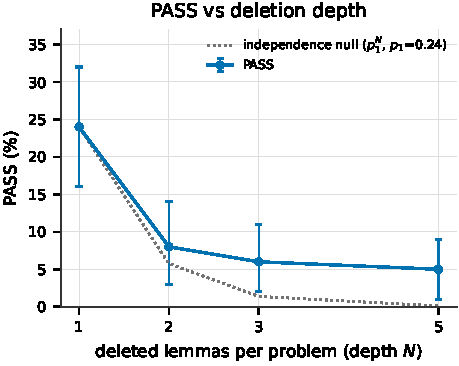
\includegraphics{deletion-curve.pdf}
  \caption{PASS versus deletion count for \texttt{claude-sonnet-5} at a 50-turn budget
  on the same 100 file--corollary pairs, compile-validated at every depth. Rates are
  per-problem, with bootstrap 95\% intervals over the 100 problems. The dotted $p_1^N$
  curve is a descriptive independence reference, not a test that distinguishes retrieval
  from derivation; the depth-2 interval contains it, so the gap at that depth is not
  resolved by this sample.}
  \label{fig:sweep}
\end{figure}

\subsection{Verbatim recall probe}
\label{sec:recall}

The probe supplies the repository, the revision, the file path and the deleted lemma's full
declaration header, withholds the proof body, and asks for the body. The cut between what is
shown and what is requested is the signature's \texttt{:=}: the model sees the docstring,
attributes, binders and statement --- what a reader of the file would have, minus the proof ---
and the ground truth is the text following \texttt{:=}, usually a \texttt{by} block. Each probe
is single-shot, with no tools and no access to the repository, so a reproduced body cannot have
been retrieved during the probe. The paired sample deletes the same lemma on both sides of a
pair, so recall is a property of the lemma; it is measured once per model and joined to the
outcomes of both holing strategies.

This addresses the knowledge-level exposure that ablation does not defeat by construction.
Instance-level exposure is already excluded, since the holed file never existed before we
made it; whether a model separately knows the lemma is the open question, and reciting a
proof body it was never shown is the one observation that would settle it affirmatively.

The probe predates the \texttt{claude-opus-5} arm and covers the other three models only;
its 339 probes are 113 lemmas each.
Table~\ref{tab:recall-scores} reports exact agreement after whitespace normalization,
normalized Levenshtein similarity, and token-level F1. Exact agreement is the only
unambiguous evidence of recall and is nearly absent: 2 of 339 probes reproduce the body,
both from \texttt{gpt-5.6-sol}, and both are one-line \texttt{by simp} proofs that any model
fluent in Lean writes from the statement alone. That stratum has to be separated, because a
corpus-wide exact-match rate is otherwise dominated by stock one-liners. On the 96 lemmas of
113 whose bodies exceed one line --- where reproducing a specific tactic sequence token for
token is not guessable --- no model matched exactly and none reached the high-similarity
band. Mean similarity is low throughout.

\begin{table}[h]
  \caption{Verbatim recall against the original proof body, per model, over the 113 deleted
  lemmas of the paired sample. \emph{Non-trivial} restricts to the 96 lemmas whose body runs
  to more than one line after the leading \texttt{by}; the high band is similarity
  $\geq 0.9$.}
  \label{tab:recall-scores}
  \centering
  \small
  \begin{tabular}{lrrrrrr}
    \toprule
    & \multicolumn{4}{c}{All 113} & \multicolumn{2}{c}{Non-trivial (96)} \\
    \cmidrule(lr){2-5}\cmidrule(lr){6-7}
    Model & exact & mean lev. & mean tok.\ F1 & high band & exact & mean lev. \\
    \midrule
    \texttt{gpt-5.6-sol}     & 2/113 & 0.269 & 0.330 & 1.8\% & 0/96 & 0.238 \\
    \texttt{claude-sonnet-5} & 0/113 & 0.286 & 0.327 & 0.9\% & 0/96 & 0.284 \\
    \texttt{leanstral-1-5}   & 0/113 & 0.189 & 0.218 & 0.0\% & 0/96 & 0.200 \\
    \bottomrule
  \end{tabular}
\end{table}

The association between recall and success is the quantity of interest, not the recall rate
on its own. Table~\ref{tab:recall-corr} gives the point-biserial correlation between recall
similarity and the same model's PASS outcome on the same problem, with a bootstrap interval
and a permutation $p$-value. Five of the six model--strategy comparisons are consistent with
no association. The sixth, \texttt{claude-sonnet-5} under whole-body holing, is positive
($r = +0.226$, $p = 0.017$) and survives controlling for proof size ($+0.215$), but it is one
result among six comparisons on a shared set of problems, it would not survive a correction
for those six, and the same model's leaf-holing estimate does not reach significance. Pass rate stratified by recall band adds nothing here:
the high band contains one or two problems per model, so its intervals span most of the unit
interval.

\begin{table}[h]
  \caption{Recall similarity against solve outcome, same model on both sides. $r$ is the
  point-biserial correlation with the PASS indicator over scorable problems, with a bootstrap
  95\% interval and a permutation $p$-value; the last column partials out proof size.}
  \label{tab:recall-corr}
  \centering
  \small
  \begin{tabular}{llrrrrr}
    \toprule
    Model & Strategy & $n$ & PASS & $r$ & 95\% CI & partial $r$ \\
    \midrule
    \texttt{gpt-5.6-sol}     & leaf  & 109 & 53 & $+0.003$ & $[-0.180, +0.197]$ & $+0.085$ \\
    \texttt{gpt-5.6-sol}     & whole & 109 & 51 & $-0.014$ & $[-0.194, +0.180]$ & $+0.098$ \\
    \texttt{claude-sonnet-5} & leaf  & 109 & 31 & $+0.157$ & $[-0.033, +0.343]$ & $+0.152$ \\
    \texttt{claude-sonnet-5} & whole & 109 & 31 & $+0.226$ & $[+0.030, +0.413]$ & $+0.215$ \\
    \texttt{leanstral-1-5}   & leaf  & 108 & 31 & $+0.042$ & $[-0.177, +0.248]$ & $+0.048$ \\
    \texttt{leanstral-1-5}   & whole & 109 & 30 & $+0.006$ & $[-0.212, +0.214]$ & $+0.015$ \\
    \bottomrule
  \end{tabular}
\end{table}

The probe finds no evidence that success on this sample is retrieval: the models that solve
these problems cannot recite the proofs they solve. A null result is weaker than its
converse would have been, and it is bounded in the obvious ways --- 113 lemmas, one prompt
format, one sample per probe, and no claim about equivalent content published elsewhere.
The interpretive caution runs in both directions. Predictable statements and easier lemmas
can support recall-like output and successful derivation at once, so even the one positive
association we found does not demonstrate training exposure.

\section{Broader impacts}
\label{app:impacts}

The corpus is proof code redistributed from public repositories under
the licenses surveyed in Appendix~\ref{app:licensing}; it contains no
personal data and no dual-use capability of its own. The intended
positive impact is to make machine-assisted proof engineering
measurable on realistic work, which is a prerequisite for lowering the
cost of formally verifying safety- and security-critical software. Two
risks are worth naming. First, a benchmark that is optimized against
can be gamed at the level of the \emph{statement} rather than the
proof; \S\ref{sec:grid} measures exactly this, and the guard of
\S\ref{sec:tampercheck} is a partial mitigation that we recommend any
verified-reward environment adopt. Second, the corpus is drawn from
projects whose authors did not release their work as an evaluation
set; we mitigate by pinning and citing every source repository at its
exact revision, surveying licenses at that revision, and flagging
rather than silently including repositories whose terms do not clearly
permit redistribution (Appendix~\ref{app:licensing}).

%%%%%%%%%%%%%%%%%%%%%%%%%%%%%%%%%%%%%%%%%%%%%%%%%%%%%%%%%%%%

\newpage
\input{checklist.tex}

\end{document}
